

%----------------------------------------------------------------------------------------
%	PACKAGES AND DOCUMENT CONFIGURATIONS
%----------------------------------------------------------------------------------------

\documentclass[a4paper,12pt]{article}
\usepackage{siunitx} % Provides the \SI{}{} and \si{} command for typesetting SI units
\usepackage{graphicx} % Required for the inclusion of images
\usepackage{subfigure}
\usepackage{multirow}
\usepackage{amsmath} % Required for some math elements 
\usepackage{indentfirst}
\usepackage{times} % Uncomment to use the Times New Roman font
\usepackage{appendix}
\usepackage{verbatim}

%----------------------------------------------------------------------------------------
%	DOCUMENT INFORMATION
%----------------------------------------------------------------------------------------

\title{ \rule{\textwidth}{0.3mm} \\UM–SJTU JOINT INSTITUTE \\ PHYSICS LABORATORY \\ (VP141) \\ \rule{\textwidth}{0.3mm} \\ [30 mm]  \Large{Laboratory Report} \\[5 mm]  Exercise 3 \\[1 mm] Simple Harmonic Motion: \\ Oscillations in Mechanical Systems\\[5 mm]} % Title
\author{Cao Zhiyuan} % Author name
\date{\today} % Date for the report

\begin{document}
\scshape

\maketitle % Insert the title, author and date

\begin{center}
\begin{tabular}{l l l}
\\[6 mm]
%Date Performed: & June 22, 2019  \\
Partners:  \\
Name: Cao Zhiyuan & ID: 518370910030 & Group: 14 \\
Name: Jiang Hang & ID: 518370910191 & Group: 1 \\
Name: Zeng Yan & ID: 518370910076 & Group: 14 \\
~\\
Date Performed:\\
June 26, 2019\\
\end{tabular}
\end{center}

\thispagestyle{empty}


\newpage


\small\tableofcontents
\thispagestyle{empty}


\newpage

%----------------------------------------------------------------------------------------
%	SECTION 1
%----------------------------------------------------------------------------------------

\setcounter{page}{1}
\upshape
\section{\textsc{Introduction}}
\subsection{\textsc{Objectives}}
In lab 3, our objective is to study the simple harmonic oscillation. First, we measure the spring constant and the effective mass of a spring. Then, we use air track to minimize the friction (external force). 
Finally, we study the relationship between oscillation period and the mass of the object. Also we find out whether the period is related to the amplitude of oscillation, and the dependence of maximum velocity on the amplitude of oscillation respectively.
\subsection{\textsc{Theoretical Background}}
One of the simplest and commonest motions in our nature is the simple harmonic motion, whose restoring force is in proportional to the displacement from the equilibrium position, and its direction is often in the opposite direction to its displacement. After analysing its free-body diagram and obtain the equation of motion, we can get the solution (the relationship between displacement $x$ and time $t$) is the sine or cosine function. Studying the simple harmonic oscillation is the foundation of learning more complicated situations.
\subsubsection{\textsc{Hooke’s Law}}
If the spring is in its elastic limit of deformation, then the force $F_x$ needed to compress or stretch the spring to the certain distance $x$ is in proportional to the very distance. The relation is called \textit{Hooke's Law}, namely:
\begin{equation}
F_x = -kx
\end{equation}
where $k$ refers to the spring constant, which describe the difficulty for it to deform the spring. To be more specific, the larger the spring constant $k$ is, the more difficult for the spring to be compressed or stretched. Also, according to the formula and Newton’s third law of dynamics, we note that the direction of the force is always in the opposite direction to the displacement, trying to put the system back into its original state, which is also the reason why the force is called restoring force. In this lab, we use \textit{Jolly balance} to measure the spring constant.
\subsubsection{\textsc{Equation of Motion of the Simple Harmonic Oscillator}}

\begin{figure}[h] 
    \centering
    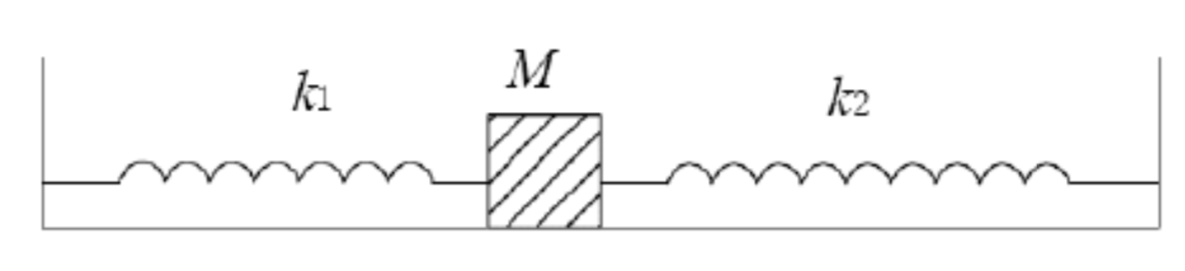
\includegraphics[width=0.5\textwidth]{Fig1} 
    \caption{The mass–spring system. \cite{labmanual}} 
\end{figure}

We start our analysis from the classical system "mass-spring system" shown in Figure 2. In the figure, an object with mass $M$ is connected by two springs with spring constant $k_1$ and $k_2$ respectively, which are measured by the Jolly balance. The object is placed on an air track, which emit gases continuously to minimize the friction force between the surface of the track and object. The origin ($x = 0$) is set to be at the equilibrium position of the mass $M$.
\par To begin with, we assume the mass of the springs can be neglected, and the damping of the system is ignored. As a result, the forces from the springs are the only forces exerted on the mass $M$. In this way, according to Newton’s second law of dynamics, the equation of motion can be written in a simple form as follows:
\begin{equation}
M\ddot{x} + (k_1 + k_2)x = 0
\end{equation}
whose general solution is:
\begin{equation}
x(t) = Acos(\omega_0 t + \varphi_0)
\end{equation}
where $A$ is the amplitude of oscillation, $\omega_0 = \sqrt{(k_1+k_2)/M}$ is the natural angular frequency of the system, and $\varphi_0$ is the initial phase. From Eq.(3), we know that the natural frequency only depends on $M$ and $k$, and has nothing to do with the initial condition, while the initial phase depends on the initial conditions. Now, we are able to calculate the period of oscillation by:
\begin{equation}
T = \frac{2\pi}{\omega_0} = 2\pi \sqrt{\frac{M}{k_1+k_2}}
\end{equation}
\par In lab 2, we will focus on the relationship between the mass $M$ of the object and its period of oscillation. 
\subsubsection{\textsc{Mass of the spring}}
Our above discussion is only an ideal situation where the mass of spring is assumed to be massless. However, in the real state, the mass of the spring cannot be neglected. In this case, we ought to take into consideration the effective mass of the spring. The effective mass of the spring $m_0$ is $1/3$ of the actual mass $m$, i.e.
\begin{equation}
m_0 = \frac{1}{3}m
\end{equation}
\par Then, the overall mass of the system is the sum of the object's mass and the effective mass of the springs, namely, the mass of the system is $M + m_0$. Hence, the angular frequency of the system can be expressed as follows:
\begin{equation}
\omega_0 = \sqrt{\frac{k_1+k_2}{M+m_0}}
\end{equation}
and thus the corresponding oscillation period is 
\begin{equation}
T = 2\pi \sqrt{\frac{M+m_0}{k_1+k_2}}
\end{equation}
\subsubsection{\textsc{Mechanical Energy in Harmonic Motion}}
We know that the potential energy of a spring is:
\begin{equation}
U = \frac{1}{2}kx^2
\end{equation}
and the kinetic energy of the mass is:
\begin{equation}
K = \frac{1}{2}Mv^2
\end{equation}
\par Because in the system, there is no non-conservative force. Therefore we are able to apply energy conservation law, i.e. 
\begin{equation}
U + K = const
\end{equation}
\par Then we analyse the system from two extreme situation. First, when the mass reaches its equilibrium position ($x = 0$), the deformation $x$ of the spring equals to $0$, therefore the potential energy $U = 0$. Also, the velocity of the mass reaches its maximum, i.e. $v_1 = v_{max}$. Hence the kinetic energy $K = K_{max}$. On the other hand, when the mass reaches its maximum displacement, i.e. $x = \pm A$, then the velocity of the mass is $v_2 = 0$ and the corresponding kinetic energy $K = 0$. Also, the potential energy of the springs reaches its maximum, namely $K = K_{max}$. Taking into account Eq.(10), we are able to conclude that:
\begin{equation}
U_{max} = K_{max}
\end{equation}
After plugging Eq.(8) and Eq.(9) into Eq.(11), we further obtain:
\begin{equation}
k = \frac{mv_{max}^2}{A^2}
\end{equation}

%----------------------------------------------------------------------------------------
%	SECTION 2
%----------------------------------------------------------------------------------------

\section{\textsc{Apparatus and Experimental Setup}}
In the first part of our experiment, we use the Jolly balance to measure the spring constant. The details are shown in Figure 2.
\par To use the Jolly balance to measure the spring constant, first we place a small mirror in the tube D and make three lines coincide with each other: the line on the mirror, the line on the tube, and the reflection in the mirror. In this way, we are able to make sure the height is accurate such that the value on the calliper is exactly the value we need. 
\begin{figure}[h] 
    \centering
    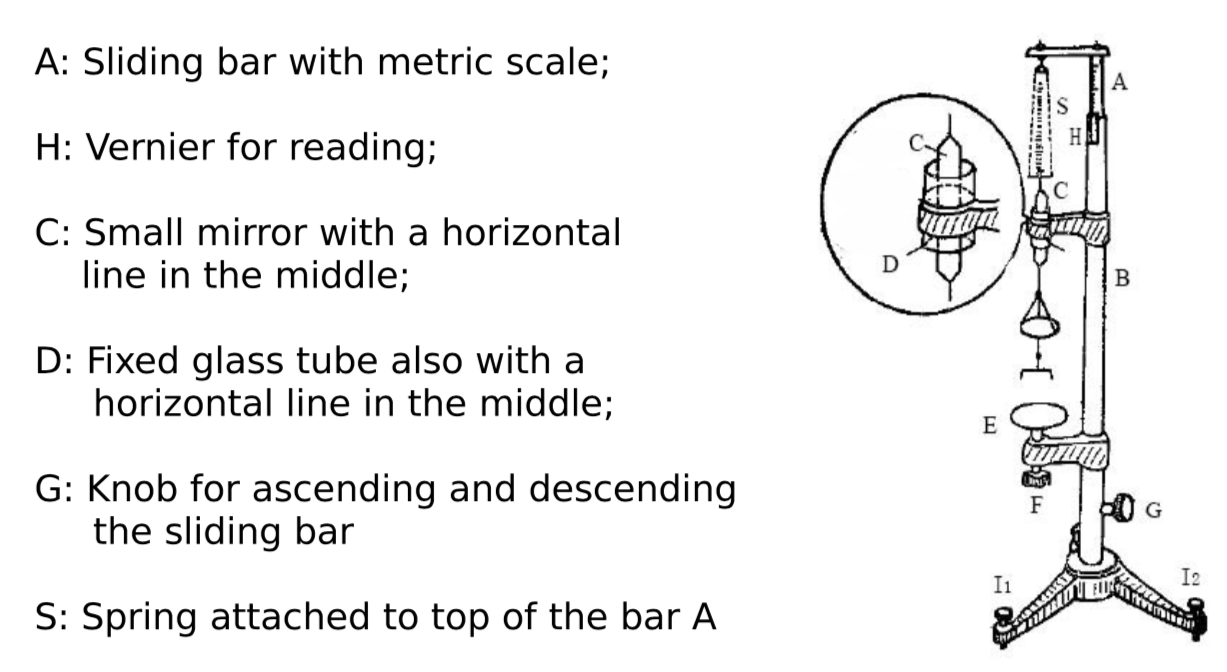
\includegraphics[width=0.7\textwidth]{Fig2} 
    \caption{Jolly balance. \cite{labmanual}} 
\end{figure}

To begin our experiment, first we don't add any weight on the spring, and make sure that the spring is parallel with the Jolly balance from two orthogonal directions. Then, we adjust knob G such that the three lines coincide. After that, read the value $L_1$.
\par Second, we add some mass $m$ on the spring, then the spring will be stretched. By adjusting knob G again, we make the three lines coincide, and record the corresponding value $L_2$. Now, we are able to find out the spring constant from the following formula:
\begin{equation}
k = \frac{mg}{L_2-L_1}
\end{equation}
\par In this lab, however, we change the value of the mass $m$ and find out the spring constant by linear fit using the least squares method\cite{labmanual}.

\begin{figure}[h] 
    \centering
    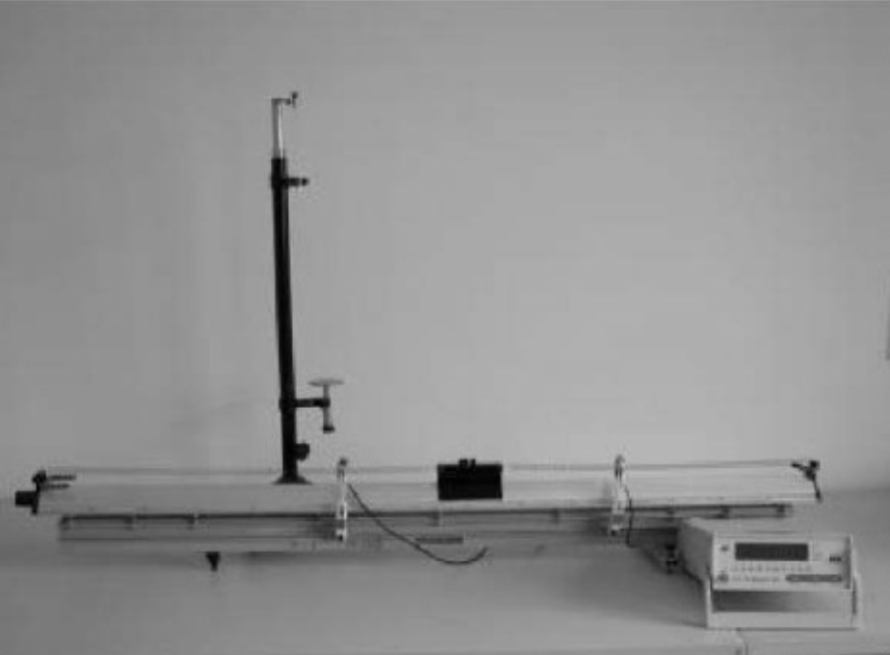
\includegraphics[width=0.5\textwidth]{Fig3} 
    \caption{The experimental setup. \cite{labmanual}} 
\end{figure}

\par The second main apparatus we use in this experiment is the photoelectric measuring system. As shown in Figure 3, the system consists of two photoelectric gates and an electronic timer. Also, there is an air track which emit gases continuously to minimize the friction between contact surfaces. When an object passes through the gate, the light will be blocked. As a result, the receiver will receive a signal and the timer begin to record the time. For period measurements, we use the I-shape shutter.

\begin{figure}[h] 
    \centering
    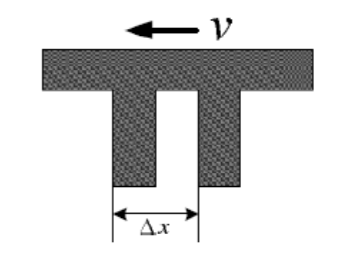
\includegraphics[width=0.25\textwidth]{Fig4} 
    \caption{The U-shape shutter. \cite{labmanual}} 
\end{figure}

\par However, when we measure the speed of an object, we use the U-shaped shutter, which is shown in Figure 4. In this way, the light will be blocked twice when the shutter passes through. Then, the time interval $\Delta t$ will be recorded. Since the distance travelled can be estimated by $\Delta x = (x_{in} + x_{out})/2$, the velocity can be estimated as:
\begin{equation}
v = \frac{\Delta x}{\Delta t} = \frac{x_{in} + x_{out}}{2\Delta t}
\end{equation}

\newpage
\par The details for the apparatus are shown in Table 1.

\begin{table}[h]
\begin{center}
\begin{tabular}{ccc}
\hline
Name of the instrument & Measured quantities & Precision \\
\hline
Timer ($T$ mode) & Time & $\pm 0.0001 [s]$ \\
Timer ($S_2$ mode) & Time & $\pm 0.00001 [s]$ \\
Electronic scale & Mass of the objects & $\pm 0.01 [g]$ \\
Calliper (Jolly balance) & Length & $\pm 0.01[cm]$ \\
Calliper & Inner and outer Distance  & $\pm 0.02 [mm]$ \\ & of the U-shape shutter \\
Ruler (Air track) & Amplitude of oscillation & $\pm 0.1 [cm]$ \\
\hline
\end{tabular}
\end{center}
\caption{Details and precisions of the apparatus.}
\end{table}

%----------------------------------------------------------------------------------------
%	SECTION 3
%----------------------------------------------------------------------------------------
\section{\textsc{Measurement Procedures}}
\subsection{\textsc{Spring Constant}}
To begin our measurement, we use the Jolly balance to find out the spring constant. First, we warm up and make some preparations for the measurement. We place the spring and mirror, and add a $20g$ preload. Then we move the knobs to make sure the mirror can be adjusted freely. After that, we check whether the spring is parallel to the balance by observing the system from two orthogonal directions. If they are not parallel, we make some adjustments on the knobs to let them coincide.
\par Second, we adjust knob G to make the three lines coincide with each other. Also, the height of the balance should be adjusted such that the initial position $L_0 = 5 [cm] \sim 10 [cm]$, and record the value $L_1$.
\par Third, we add mass $m_1$ and record length $L_1$, and after that, we keep adding another mass $m_2$ and record $L_2$. After repeating the process for six times, we collect six data. Note that the order of the masses should be recorded.
\par Fourth, the spring constant $k_1$ can be estimated by plotting a linear fit with least squares method.
\par Lastly, change another spring and use the same method to find out the spring constant $k_2$. And then attach spring 1 and spring 2 together with preload removed. We are able to compare $k_3$ with theories.

\subsection{\textsc{Relation Between the Oscillation Period T and the Mass of the Oscillator M}}
\subsubsection{\textsc{Early-stage adjustments}}
First, we check that the air track is horizontal. Then, we turn on the track and examine whether any hole is blocked. After that, we place the cart on the track, and by adjusting the single knob on the track, we make sure that the cart can move slowly back and forth. Note that before the air pump is turned on, no object is allowed to be placed on the track. Otherwise the track may deform, and the scales on it will be inaccurate.
\subsubsection{\textsc{Horizontal air track}}
In this part, we focus on the horizontal track. To begin with, we attach the springs to both sides of the track and use the I-shape shutter. Also, we should pay attention to the photoelectric gate so that it is in its equilibrium position.
\par Then, we begin our experiment. We place a mass $m_1$ on the cart and make it oscillate between the equilibrium position at an amplitude $A = 5 [cm]$ with the help of a ruler. Then, we release the car and set the timer as the "T" mode. The timer will automatically record the 10 periods of the oscillation. Record the mass and time period.
\par After that, we add some more weights on the cart, and repeat the procedure for 5 times. Finally, since  other factors remain the same, we plot a linear fit to analyse the relationship between M and T.  
\subsubsection{\textsc{Inclined air track}}
Actually, inclination of the track may also influence the oscillation period. To change the inclination of the air track, we put some plastic plates under it. In this lab, we place 3 and 6 plates respectively and repeat the steps in (3.2.2). Finally, we plot a linear fit to discuss the relationship between M and T.

\subsection{\textsc{Relation Between the Oscillation Period T and the Amplitude A}}
In this part, we study the relationship between period $T$ and Amplitude $A$. We keep other factors unchanged and only change the amplitude. By choosing 6 different values (such as 5.0/ 10.0/ 15.0 [cm]...), we will obtain six groups of data. 
\par Finally, we apply a linear fit to the data, and find out the dependence of period $T$ on amplitude $A$ with a correlation coefficient $\gamma$.

\subsection{\textsc{Relation Between the Maximum Speed and the Amplitude}}
In this part, we measure the dependence of maximum speed on the amplitude. First, we change the shutter to the U-shaped one and select the "$S_2$" mode. Then the period interval $\Delta t$ can be automatically recorded. Since the outer distance and the inner distance $x_{in}$ and $x_{out}$ can be measured by the calliper, the overall distance can be estimated as $\Delta x = (x_{in} + x_{out})/2$. Thus the maximum speed can be calculated accordingly.
\par After that, we change the amplitude of oscillation and we collect six data for different A (the recommended values are 5.0/ 10.0/ 15.0 [cm]...). Eventually, with the help of Eq.(12), we find out the $v_{max}$ and compare the result.

\subsection{\textsc{Mass measurement}}
In experiment 3, there are many masses we need to measure. When using the electronic scale, adjust it to be horizontal every time we use it. And when measuring the weight, we put them together. For instance, we measure the mass of the cart and the load together, which enables us to minimize the uncertainties which will otherwise occur when adding the masses together. Besides, note that we should begin our measurement before the circular symbol on the scale disappear.


%----------------------------------------------------------------------------------------
%	SECTION 4
%----------------------------------------------------------------------------------------
\section{\textsc{Results}}
\subsection{\textsc{Mass Measurement}}
In this lab, we obtain most of our results based on mass. Hence at first we analyse the mass involved. The data are recorded in Table 1 and Table 2 .

\setlength{\tabcolsep}{7mm}{
\begin{table}[h]
\begin{center}
\begin{tabular}{|c|c|c|}
\hline
\multicolumn{3}{|c|}{m [g] $\pm$ 0.01 [g]} \\
\hline
1 & $\sum_{i=1}^1 m_i$ & 4.70 \\
2 & $\sum_{i=1}^2 m_i$ & 9.41 \\
3 & $\sum_{i=1}^3 m_i$ & 14.17 \\
4 & $\sum_{i=1}^4 m_i$ & 19.01 \\
5 & $\sum_{i=1}^5 m_i$ & 23.81 \\
6 & $\sum_{i=1}^6 m_i$ & 28.61 \\
\hline
\end{tabular}
\end{center}
\caption{The mass of loads.}
\end{table}
}
where $m_i$ refers to the $i^{th}$ mass added to the cart.

\begin{table}[h]
\begin{center}
\begin{tabular}{|c|c|}
\hline
\multicolumn{2}{|c|}{m [g] $\pm$ 0.01 [g]} \\
\hline
Object with I-shape shutter $m_I$ & ~~~~~~177.22~~~~~~ \\
Object with U-shape shutter $m_U$ & 185.37 \\
Mass of Spring 1 \& 2 $m_{spr1,2}$ & 21.31 \\
\hline
\end{tabular}
\end{center}
\caption{The mass of objects.}
\end{table}

\newpage
Based on Table 3, we can calculate the equivalent mass and their uncertainties, and the results are shown as follows (The detailed calculations are involved in Appendix A.1):
      \begin{center}
      $ \displaystyle M_I = m_I + \frac{1}{3}m_{spr1,2} = 184.327 [g] \pm 0.011 [g] ~~~~~~ u_{rM_I} = 0.006\%$
      \end{center}
      \begin{center}
      $ \displaystyle M_U = m_U + \frac{1}{3}m_{spr1,2} = 192.477 [g] \pm 0.011 [g] ~~~~~~ u_{rM_U} = 0.006\%$
      \end{center}
      
      
\subsection{\textsc{Spring Constant}}
We begin our experiment by using the Jolly balance to measure the spring constant. Then we record the different $L$ corresponding to different loads. The data are recorded in Table 4.

\begin{table}[h]
\begin{center}
\resizebox{\textwidth}{20mm}{
\begin{tabular}{|c|c||c|c||c|c|}
\hline
\multicolumn{2}{|c||}{spring 1 [cm] $\pm$ 0.01 [cm]} & \multicolumn{2}{|c||}{spring 2 [cm] $\pm$ 0.01 [cm]} & \multicolumn{2}{|c|}{series [cm] $\pm$ 0.01 [cm]}\\
\hline
$L_0$ & 6.03 & $L_0$ & 5.69 & $L_0$ & 9.84 \\
$L_1$ & 8.08 & $L_1$ & 7.55 & $L_1$ & 13.58 \\
$L_2$ & 10.09 & $L_2$ & 9.45 & $L_2$ & 17.58 \\
$L_3$ & 12.30 & $L_3$ & 11.37 & $L_3$ & 21.54\\
$L_4$ & 14.50 & $L_4$ & 13.25 & $L_4$ & 25.65 \\
$L_5$ & 16.69 & $L_5$ & 15.18 & $L_5$ & 29.66\\
$L_6$ & 18.83 & $L_6$ & 17.10 & $L_6$ & 33.81\\
\hline
\end{tabular}
}
\end{center}
\caption{Measurement for single constant.}
\end{table}

\par Then, we are able to obtain the change of length $\Delta L$ by the following formula:
\begin{center}
$ \Delta L_i = L_i - L_0 $
\end{center}
where $i = 1,2,3,4,5,6$. Now we are able to obtain the $\Delta L$ for each set of data, and their uncertainties can be calculated as follows (The detailed calculations are shown in Appendix A.2). We take spring 1 as an example:
\begin{center}
$ \Delta L_1 = L_1 - L_0 = 2.050 [cm] \pm  0.014 [cm]$ ~~~~~~ $ u_{\Delta L_1} = 0.7 \% $
\end{center}
The rest of the data can be calculated in exact the same way, and the overall data with their uncertainties are recorded in Table 5, Table 6, and Table 7.

\begin{table}[h]
\begin{center}
\begin{tabular}{|c|c|c|c|}
\hline
spring 1 &$ \Delta L $ [cm]  & $ u_{\Delta L_i} $ [cm] & $ u_{r\Delta L_i} $\\
\hline
$\Delta L_1$ & 2.050 & 0.014 & 0.7\% \\
$\Delta L_2$ & 4.060 & 0.014 & 0.3\% \\
$\Delta L_3$ & 6.270 & 0.014 & 0.2\% \\
$\Delta L_4$ & 8.470 & 0.014 & 0.17\% \\
$\Delta L_5$ & 10.660 & 0.014 & 0.13\%\\
$\Delta L_6$ & 12.800 & 0.014 & 0.11\% \\
\hline
\end{tabular}
\end{center}
\caption{Uncertainties for spring 1.}
\end{table}

\begin{table}[h]
\begin{center}
\begin{tabular}{|c|c|c|c|}
\hline
spring 1 &$ \Delta L $ [cm]  & $ u_{\Delta L_i} $ [cm] & $ u_{r\Delta L_i} $\\
\hline
$\Delta L_1$ & 1.860 & 0.014 & 0.8\% \\
$\Delta L_2$ & 3.760 & 0.014 & 0.4\% \\
$\Delta L_3$ & 5.880 & 0.014 & 0.2\% \\
$\Delta L_4$ & 7.560 & 0.014 & 0.19\% \\
$\Delta L_5$ & 9.490 & 0.014 & 0.15\%\\
$\Delta L_6$ & 11.410 & 0.014 & 0.12\% \\
\hline
\end{tabular}
\end{center}
\caption{Uncertainties for spring 2.}
\end{table}

\begin{table}[p]
\begin{center}
\begin{tabular}{|c|c|c|c|}
\hline
spring 1 &$ \Delta L $ [cm]  & $ u_{\Delta L_i} $ [cm] & $ u_{r\Delta L_i} $\\
\hline
$\Delta L_1$ & 3.740 & 0.014 & 0.4\% \\
$\Delta L_2$ & 7.740 & 0.014 & 0.18\% \\
$\Delta L_3$ & 11.700 & 0.014 & 0.12\% \\
$\Delta L_4$ & 15.810 & 0.014 & 0.09\% \\
$\Delta L_5$ & 19.820 & 0.014 & 0.07\%\\
$\Delta L_6$ & 23.970 & 0.014 & 0.06\% \\
\hline
\end{tabular}
\end{center}
\caption{Uncertainties for spring series.}
\end{table}

\newpage
From the mass we have calculated in 4.1, we have:
\begin{center}
$ u_m = 0.010 [g] $
\end{center}
Therefore, we are able to obtain that (The detailed calculations are shown in Appendix A.2): 
\begin{center}
$ u_{mg} = u_G = 0.00010 [N]$
\end{center}

\par Now, we are able to use \textit{Origin} to plot the linear fit for them. The results are shown in Figure 5, Figure 6, and Figure 7.

\begin{figure}[p] 
    \centering
    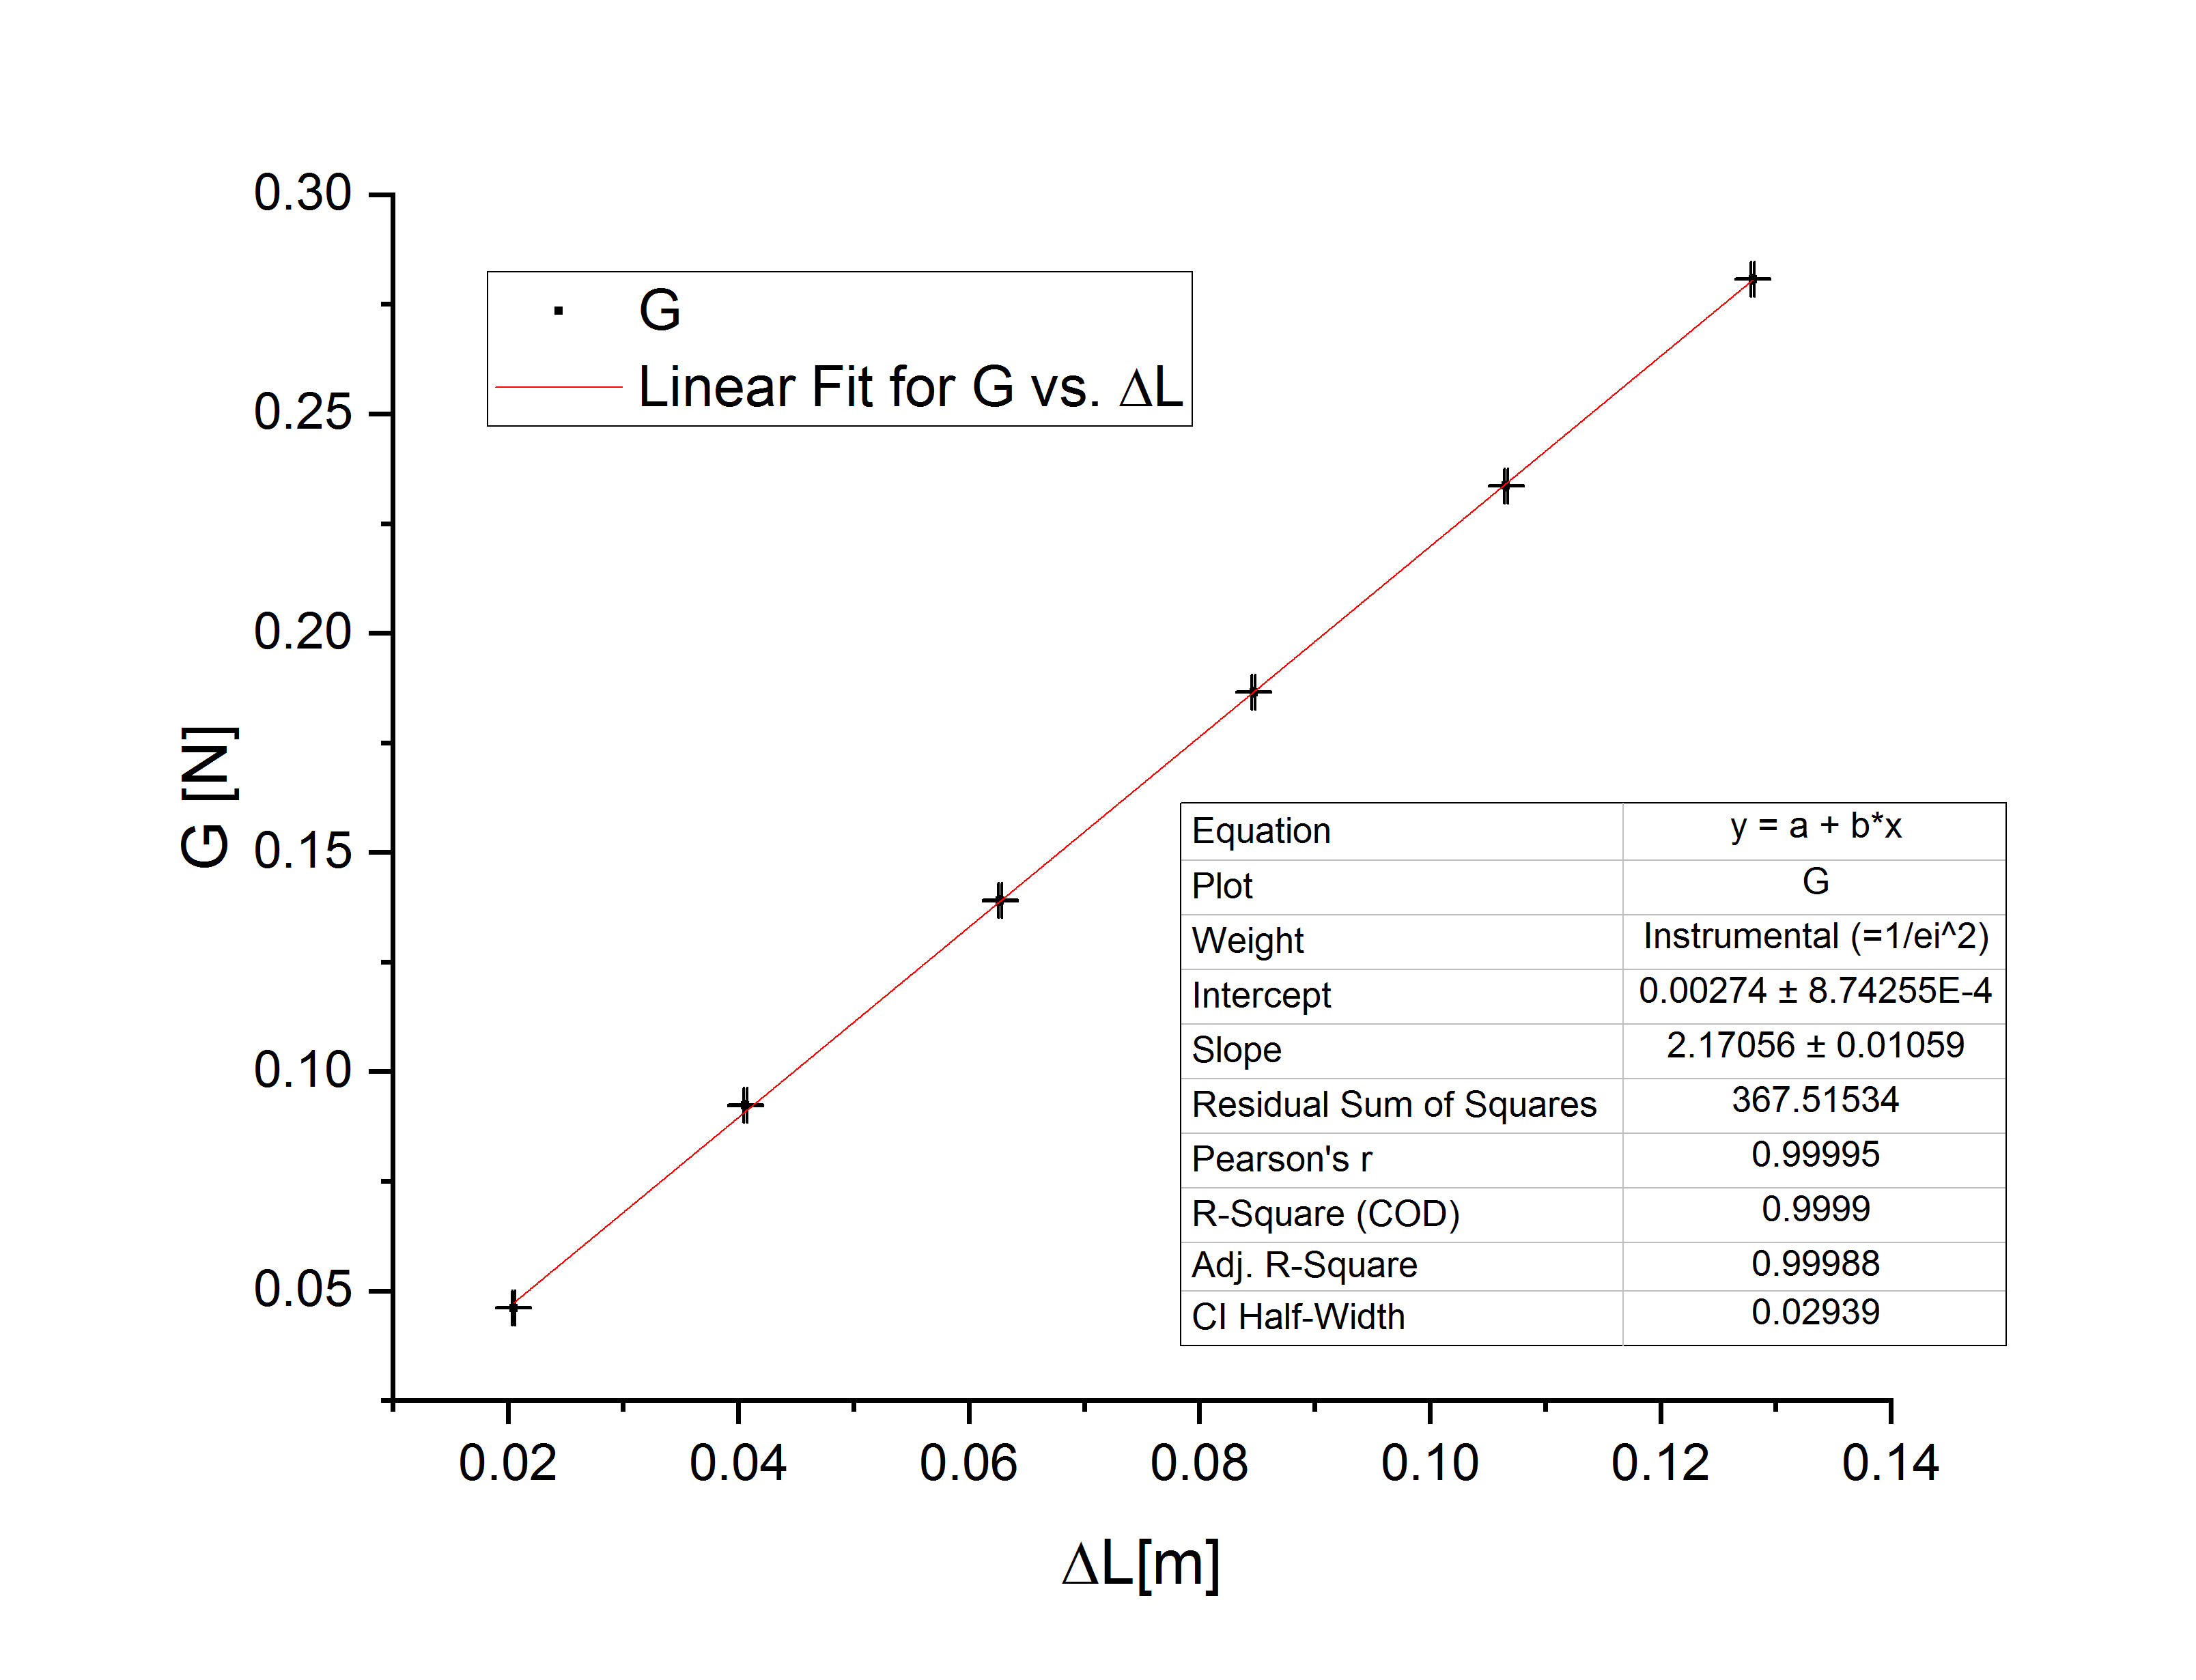
\includegraphics[width=1\textwidth]{pic1} 
    \caption{Linear Fit for spring 1.} 
\end{figure}

\begin{figure}[p] 
    \centering
    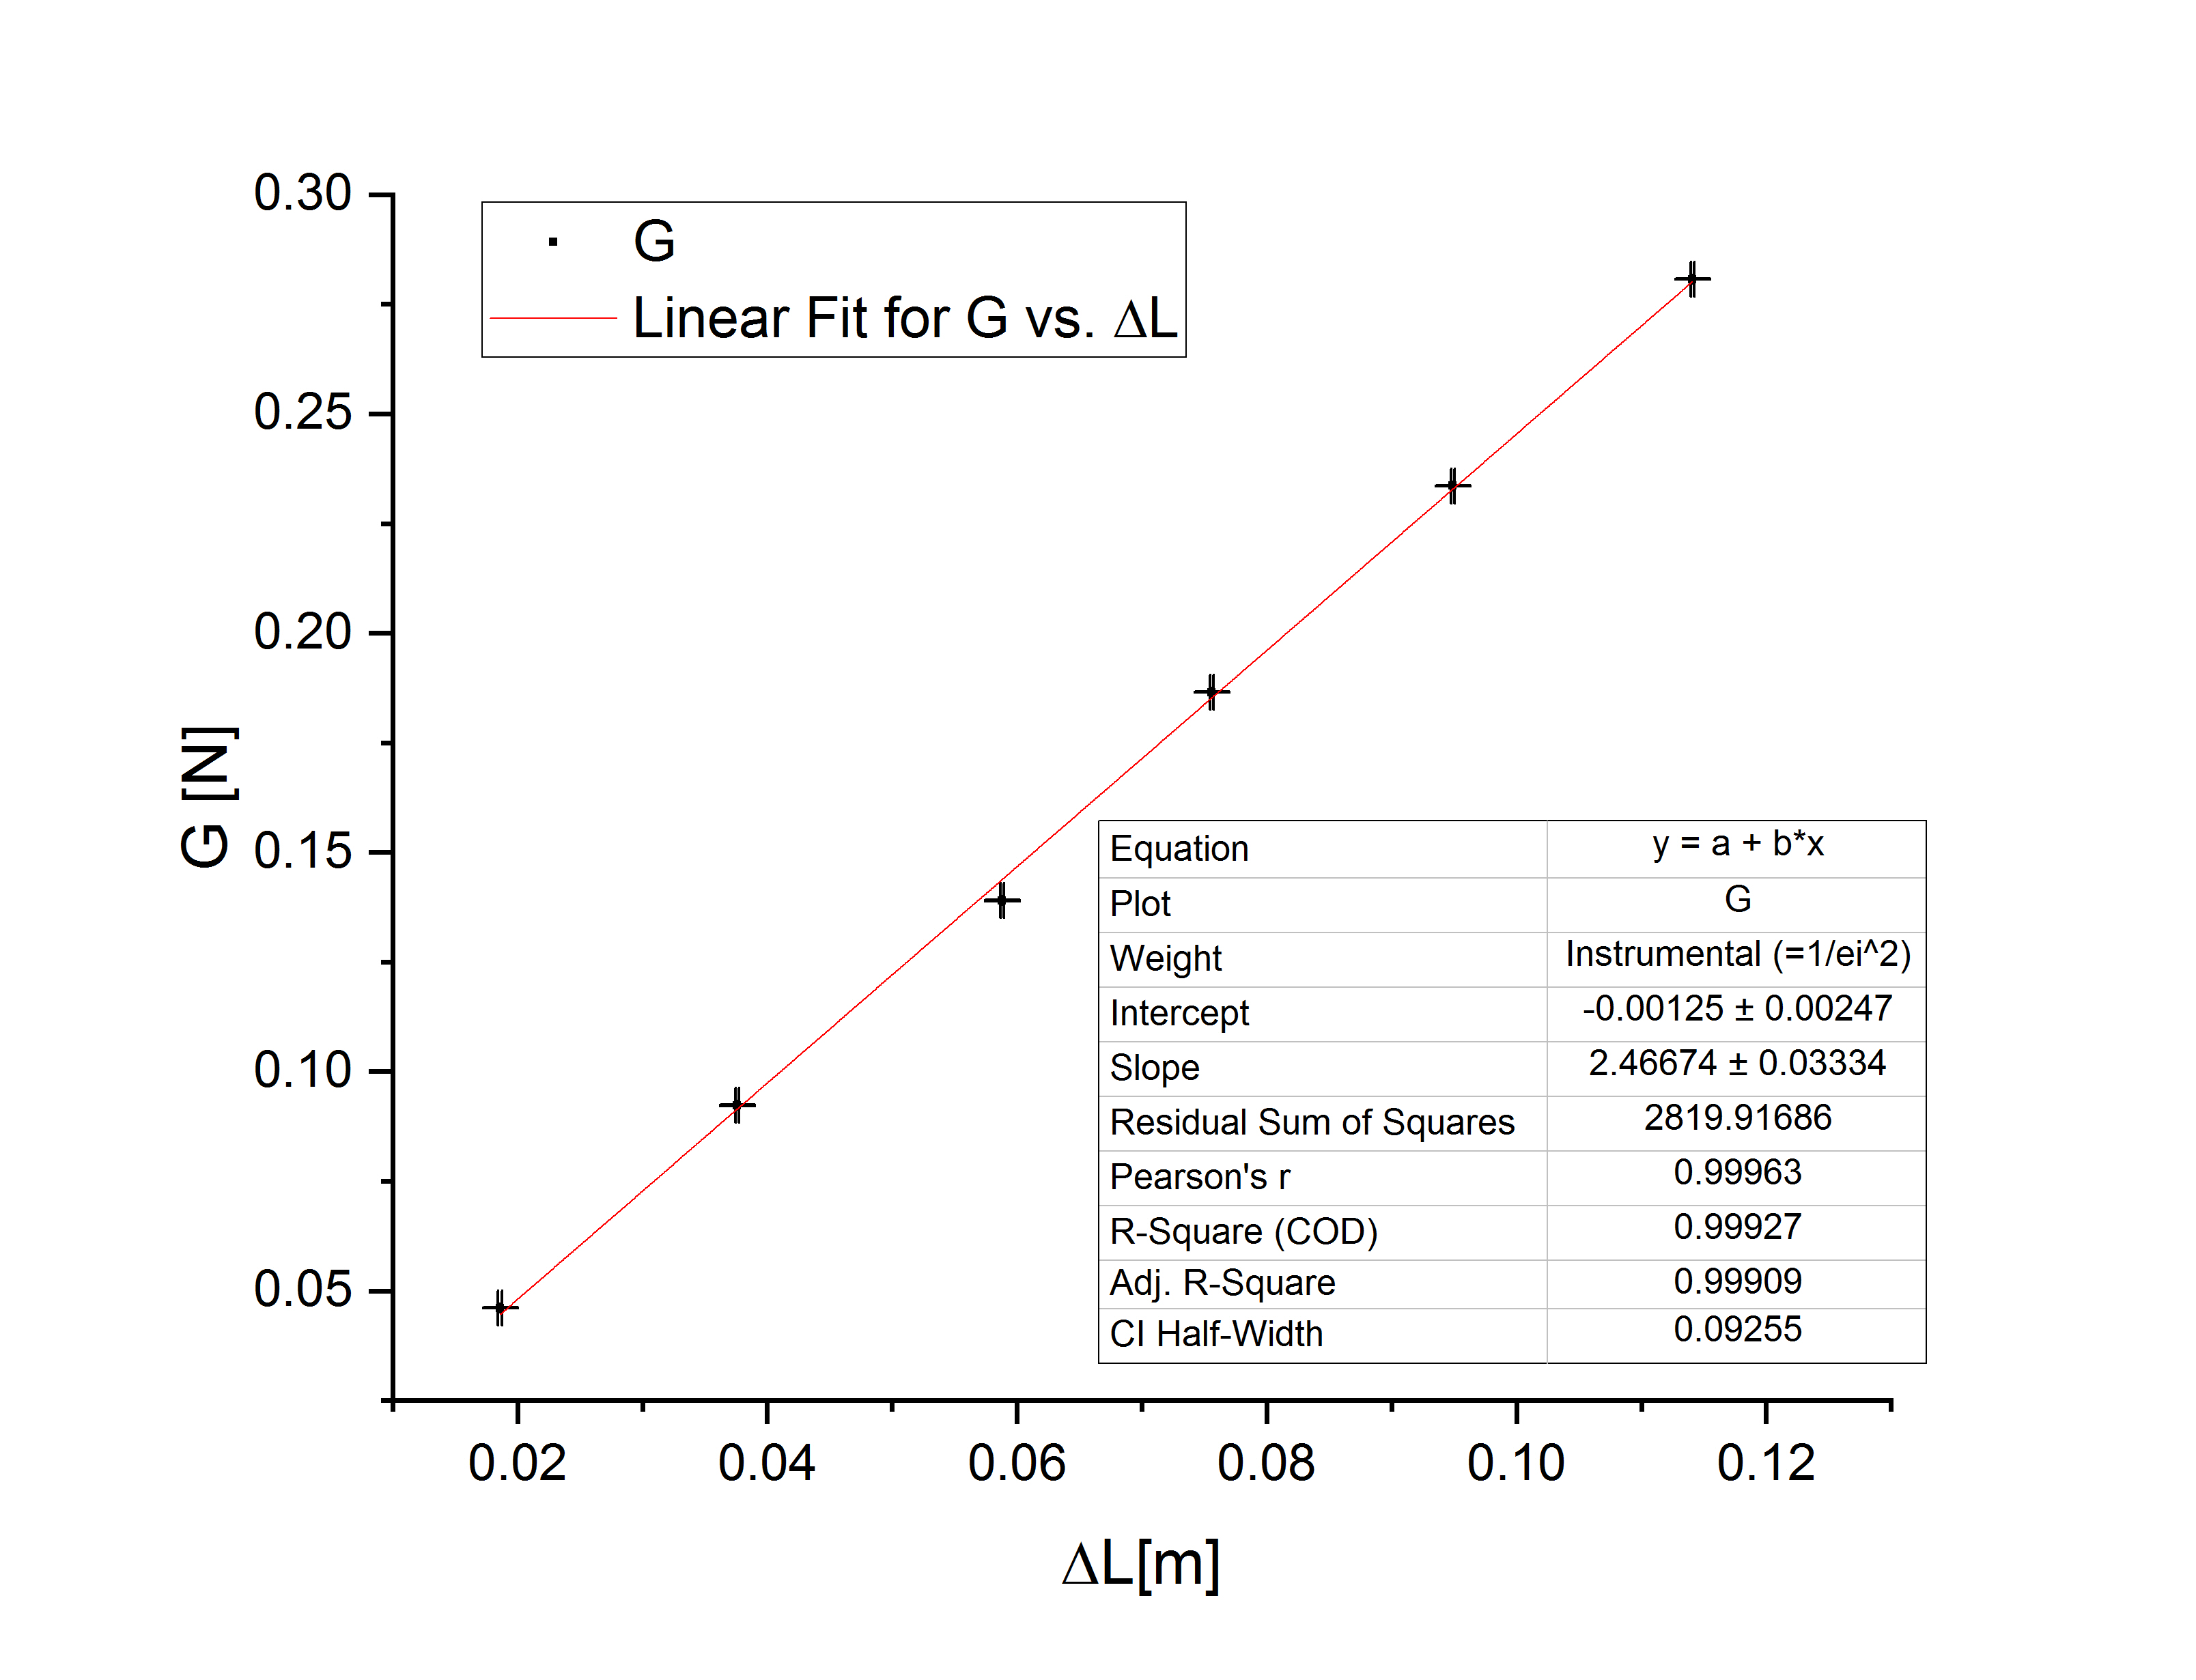
\includegraphics[width=1\textwidth]{pic2} 
    \caption{Linear Fit for spring 2.} 
\end{figure}

\begin{figure}[p] 
    \centering
    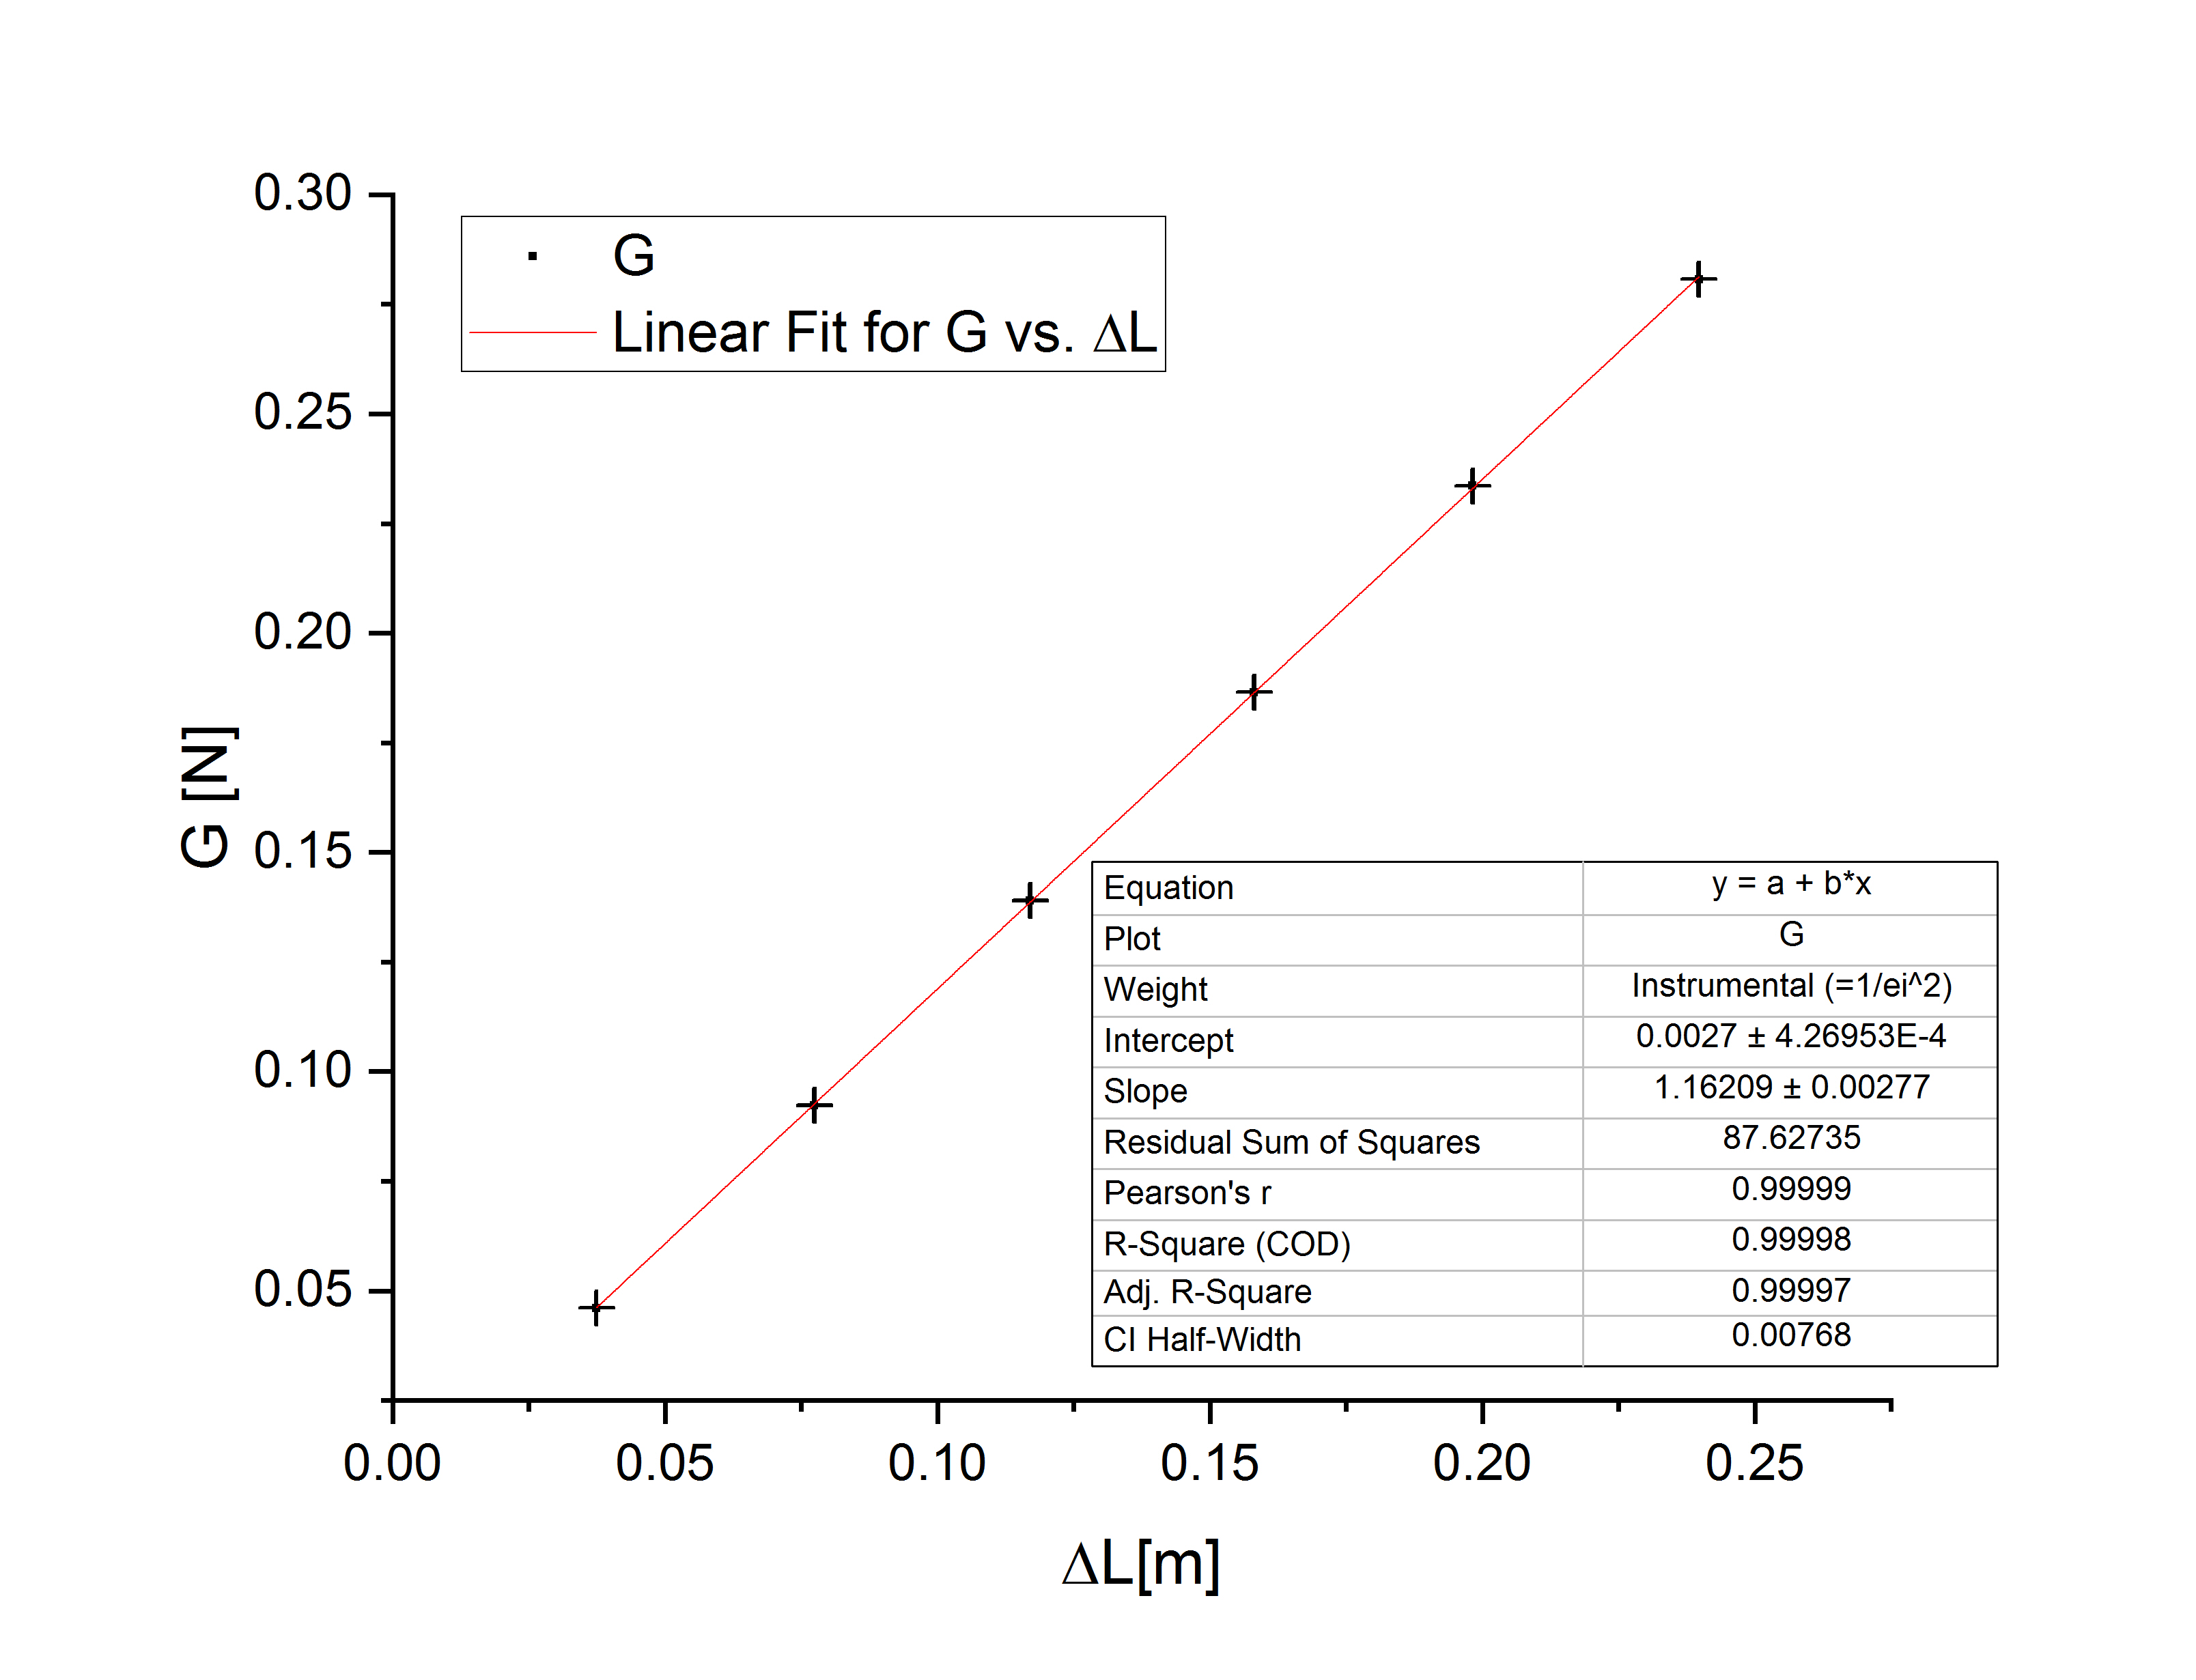
\includegraphics[width=1\textwidth]{pic3} 
    \caption{Linear Fit for spring series.} 
\end{figure}

It can be seem that from Eq.(1), we have $mg = k\Delta l$. Therefore, we obtain the spring constants from the following graphs. The uncertainties are the CI Half-Width, which are shown in the last row of the attached table of each graph. Based on the figures, we obtain the spring constants as follows:
\begin{center}
$ k_1 = 2.17 [N/m] \pm 0.03 [N/m] $ ~~~~~~ $ u_{k1} = 1.4\% $
\end{center}
\begin{center}
$ k_2 = 2.47 [N/m] \pm 0.09 [N/m] $ ~~~~~~ $ u_{k2} = 4\% $
\end{center}
\begin{center}
$ k_s = 1.162[N/m] \pm 0.008[N/m] $ ~~~~~~ $ u_{ks} = 0.7\% $
\end{center}

\par Then, we check the theoretical value $ k_{th} $ of the spring constant in series based on $k_1$ and $k_2$, and compared $k_{th}$ with our measured $k_s$. The theoretical value $k_{th}$ can be given by the following formula (The detailed calculations are involved in Appendix A.2):
\begin{center}
$\displaystyle  k_{th} = \frac{1}{1/k_1 + 1/k_2} = \frac{k_1k_2}{k_1+k_2} = 1.16 [N/m] \pm 0.02 [N/m]$
\end{center}
with a relative uncertainty:
\begin{center}
$ u_{rk_{th}} = 2\% $
\end{center}
\par Now, we are able to calculate the deviation of the experimental value between the measured value as follows:
\begin{center}
$ \displaystyle u_{r} = \frac{|k_{th} - k_s|}{k_{th}}\times 100\% = 0.17 \% $
\end{center}

\subsection{\textsc{Relation between the oscillation period T and the mass of the oscillator M}}
In this lab, we measure the dependence of period $T$ on the mass $m$, and change the inclination of the air track. The data with three different inclination are recorded in Table 8.

\begin{table}[h]
\begin{center}
\begin{tabular}{|c|c||c|c||c|c|}
\hline
\multicolumn{6}{|c|}{ten periods [s] $\pm$ 0.0001[s] } \\
\hline
\multicolumn{2}{|c||}{horizontal} & \multicolumn{2}{|c||}{incline 1 (3 disks)} & \multicolumn{2}{|c|}{incline 2 (6 disks)}\\
\hline
$m_1$ & 12.6481 & $m_1$ & 12.5973 & $m_1$ & 12.6160 \\
$m_2$ & 12.7636 & $m_2$ & 12.7657 & $m_2$ & 12.7725 \\
$m_3$ & 12.9203 & $m_3$ & 12.9330 & $m_3$ & 12.9112 \\
$m_4$ & 13.0617 & $m_4$ & 13.0699 & $m_4$ & 13.0861 \\
$m_5$ & 13.2077 & $m_5$ & 13.2258 & $m_5$ & 13.2481 \\
$m_6$ & 13.3534 & $m_6$ & 13.3807 & $m_6$ & 13.3875 \\
\hline
\end{tabular}
\end{center}
\caption{Measurement data for the T vs. M relation.}
\end{table}
\par Since in this lab, we plot a linear fit in terms of $M$ vs. $T^2$, and we already have the data of $m$ calculated in 4.1, what we need to do is to find out the values of $T^2$ and their corresponding uncertainties. The general formula for obtaining $T^2$ can be written as follows:
\begin{center}
$\displaystyle T^2 = (\frac{T_{0,i}}{10})^2 = \frac{T_{0,i}^2}{100}$
\end{center}
Then, we are able to calculate its value and corresponding uncertainty (The detailed calculations are shown in Appendix A.3). The data are shown in Table 8, Table 9, and Table 10.

\begin{table}[h]
\begin{center}
\begin{tabular}{|c|c|c|c|}
\hline
Horizontal & $T_i^2 [s^2] $ & $u_{{T_i}^2} [s^2] $ & $ u_{r{T_i}^2} $\\
\hline
$m_1$ & 1.59974 & 0.00003 & 0.0018\%  \\
$m_2$ & 1.62909 & 0.00003 & 0.0018\%  \\
$m_3$ & 1.66934 & 0.00003 & 0.0018\%  \\
$m_4$ & 1.70608 & 0.00003 & 0.0018\%  \\
$m_5$ & 1.74443 & 0.00003 & 0.0017\%  \\
$m_6$ & 1.78313 & 0.00003 & 0.0017\%  \\
\hline
\end{tabular}
\end{center}
\caption{Uncertainties for horizontal track.}
\end{table}

\begin{table}[h]
\begin{center}
\begin{tabular}{|c|c|c|c|}
\hline
Incline 1 & $T_i^2 [s^2] $ & $u_{{T_i}^2} [s^2] $ & $ u_{r{T_i}^2} $\\
\hline
$m_1$ & 1.58692 & 0.00003 & 0.0019\%  \\
$m_2$ & 1.62963 & 0.00003 & 0.0018\%  \\
$m_3$ & 1.67262 & 0.00003 & 0.0018\%  \\
$m_4$ & 1.70822 & 0.00003 & 0.0018\%  \\
$m_5$ & 1.74922 & 0.00003 & 0.0017\%  \\
$m_6$ & 1.79043 & 0.00003 & 0.0017\%  \\
\hline
\end{tabular}
\end{center}
\caption{Uncertainties for track with incline 1.}
\end{table}

\begin{table}[p]
\begin{center}
\begin{tabular}{|c|c|c|c|}
\hline
Incline 2 & $T_i^2 [s^2] $ & $u_{{T_i}^2} [s^2] $ & $ u_{r{T_i}^2} $\\
\hline
$m_1$ & 1.59163 & 0.00003 & 0.0019\%  \\
$m_2$ & 1.63137 & 0.00003 & 0.0018\%  \\
$m_3$ & 1.66699 & 0.00003 & 0.0018\%  \\
$m_4$ & 1.71246 & 0.00003 & 0.0018\%  \\
$m_5$ & 1.75512 & 0.00003 & 0.0017\%  \\
$m_6$ & 1.79225 & 0.00003 & 0.0017\%  \\
\hline
\end{tabular}
\end{center}
\caption{Uncertainties for track with incline 2.}
\end{table}

\par Besides, in order to plot the $M$ vs. $T^2$ linear fit, the uncertainties of masses are also needed. Based on the calculations in A.3, our uncertainties of mass is: 
\begin{center}
$ u_{M_i} = 0.015[g] = 0.000015 [kg] $
\end{center}

\par Now, with all the uncertainties involved, we are able to use \textit{Origin} to plot a $M$ vs. $T^2$ linear fit. The results are shown in Figure 8, Figure 9, and Figure 10.

\begin{figure}[p] 
    \centering
    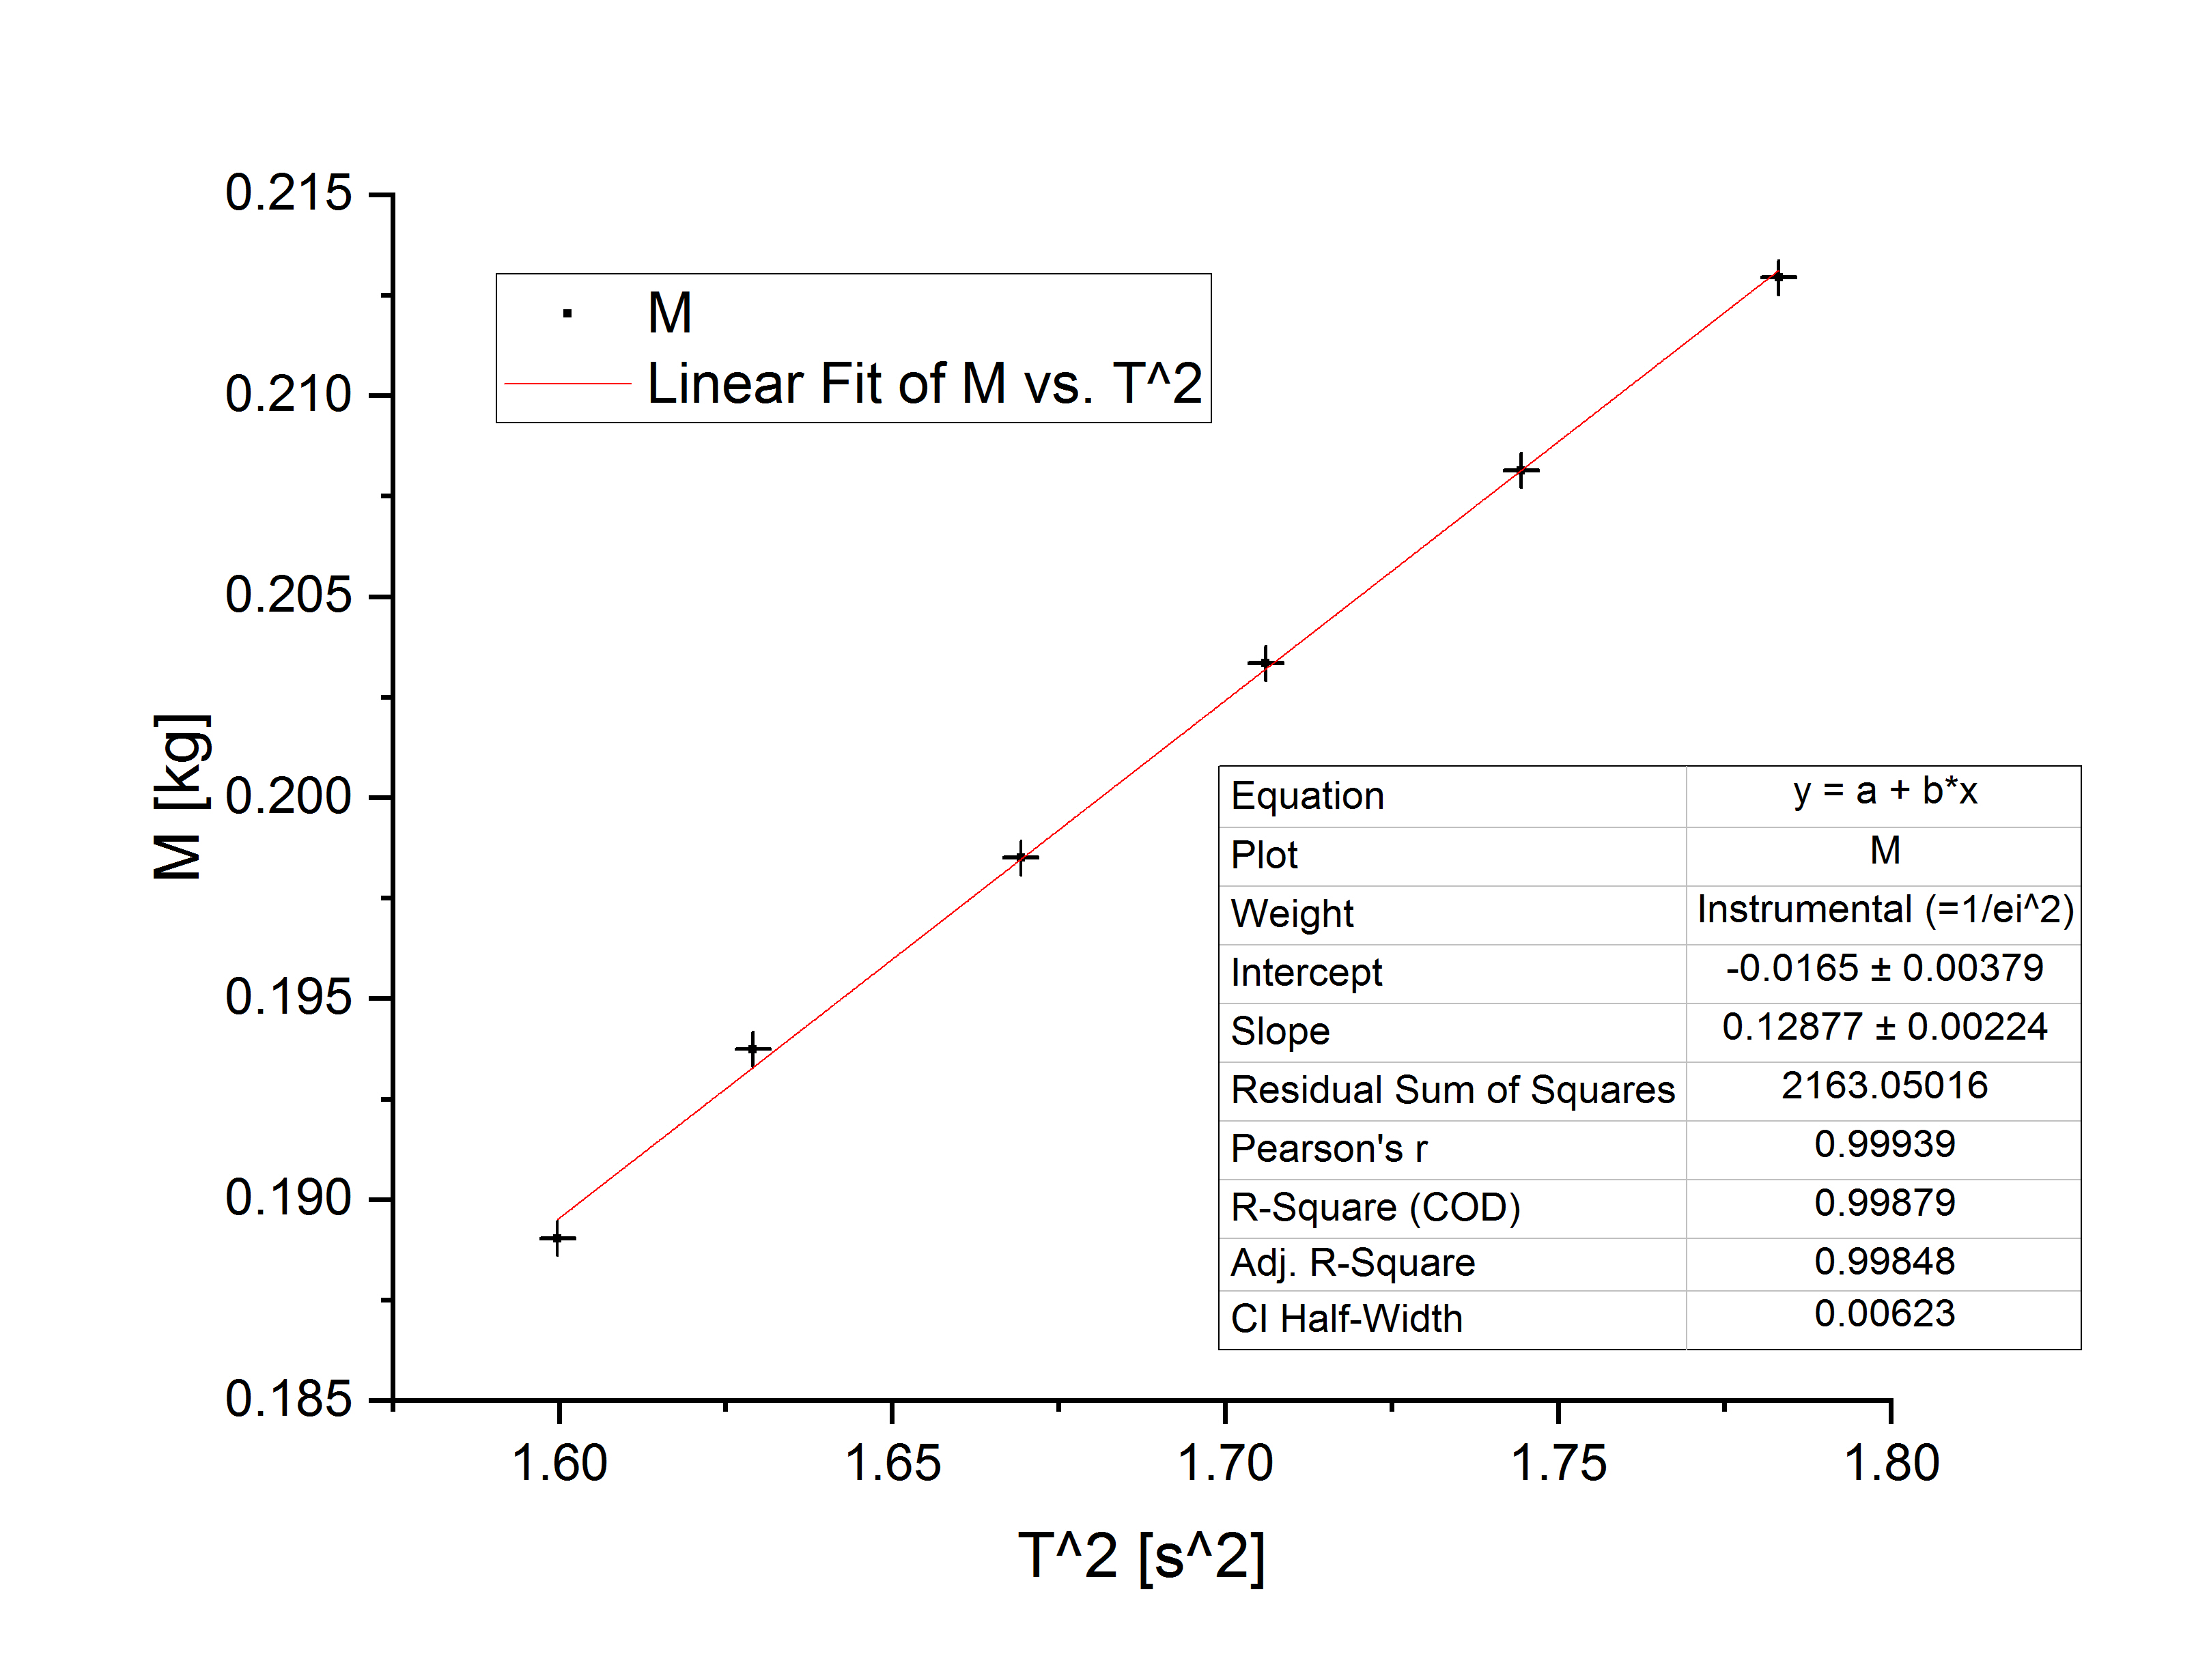
\includegraphics[width=1\textwidth]{pic4} 
    \caption{Linear Fit of $M$ vs. $T^2$ (horizontal).} 
\end{figure}

\begin{figure}[p] 
    \centering
    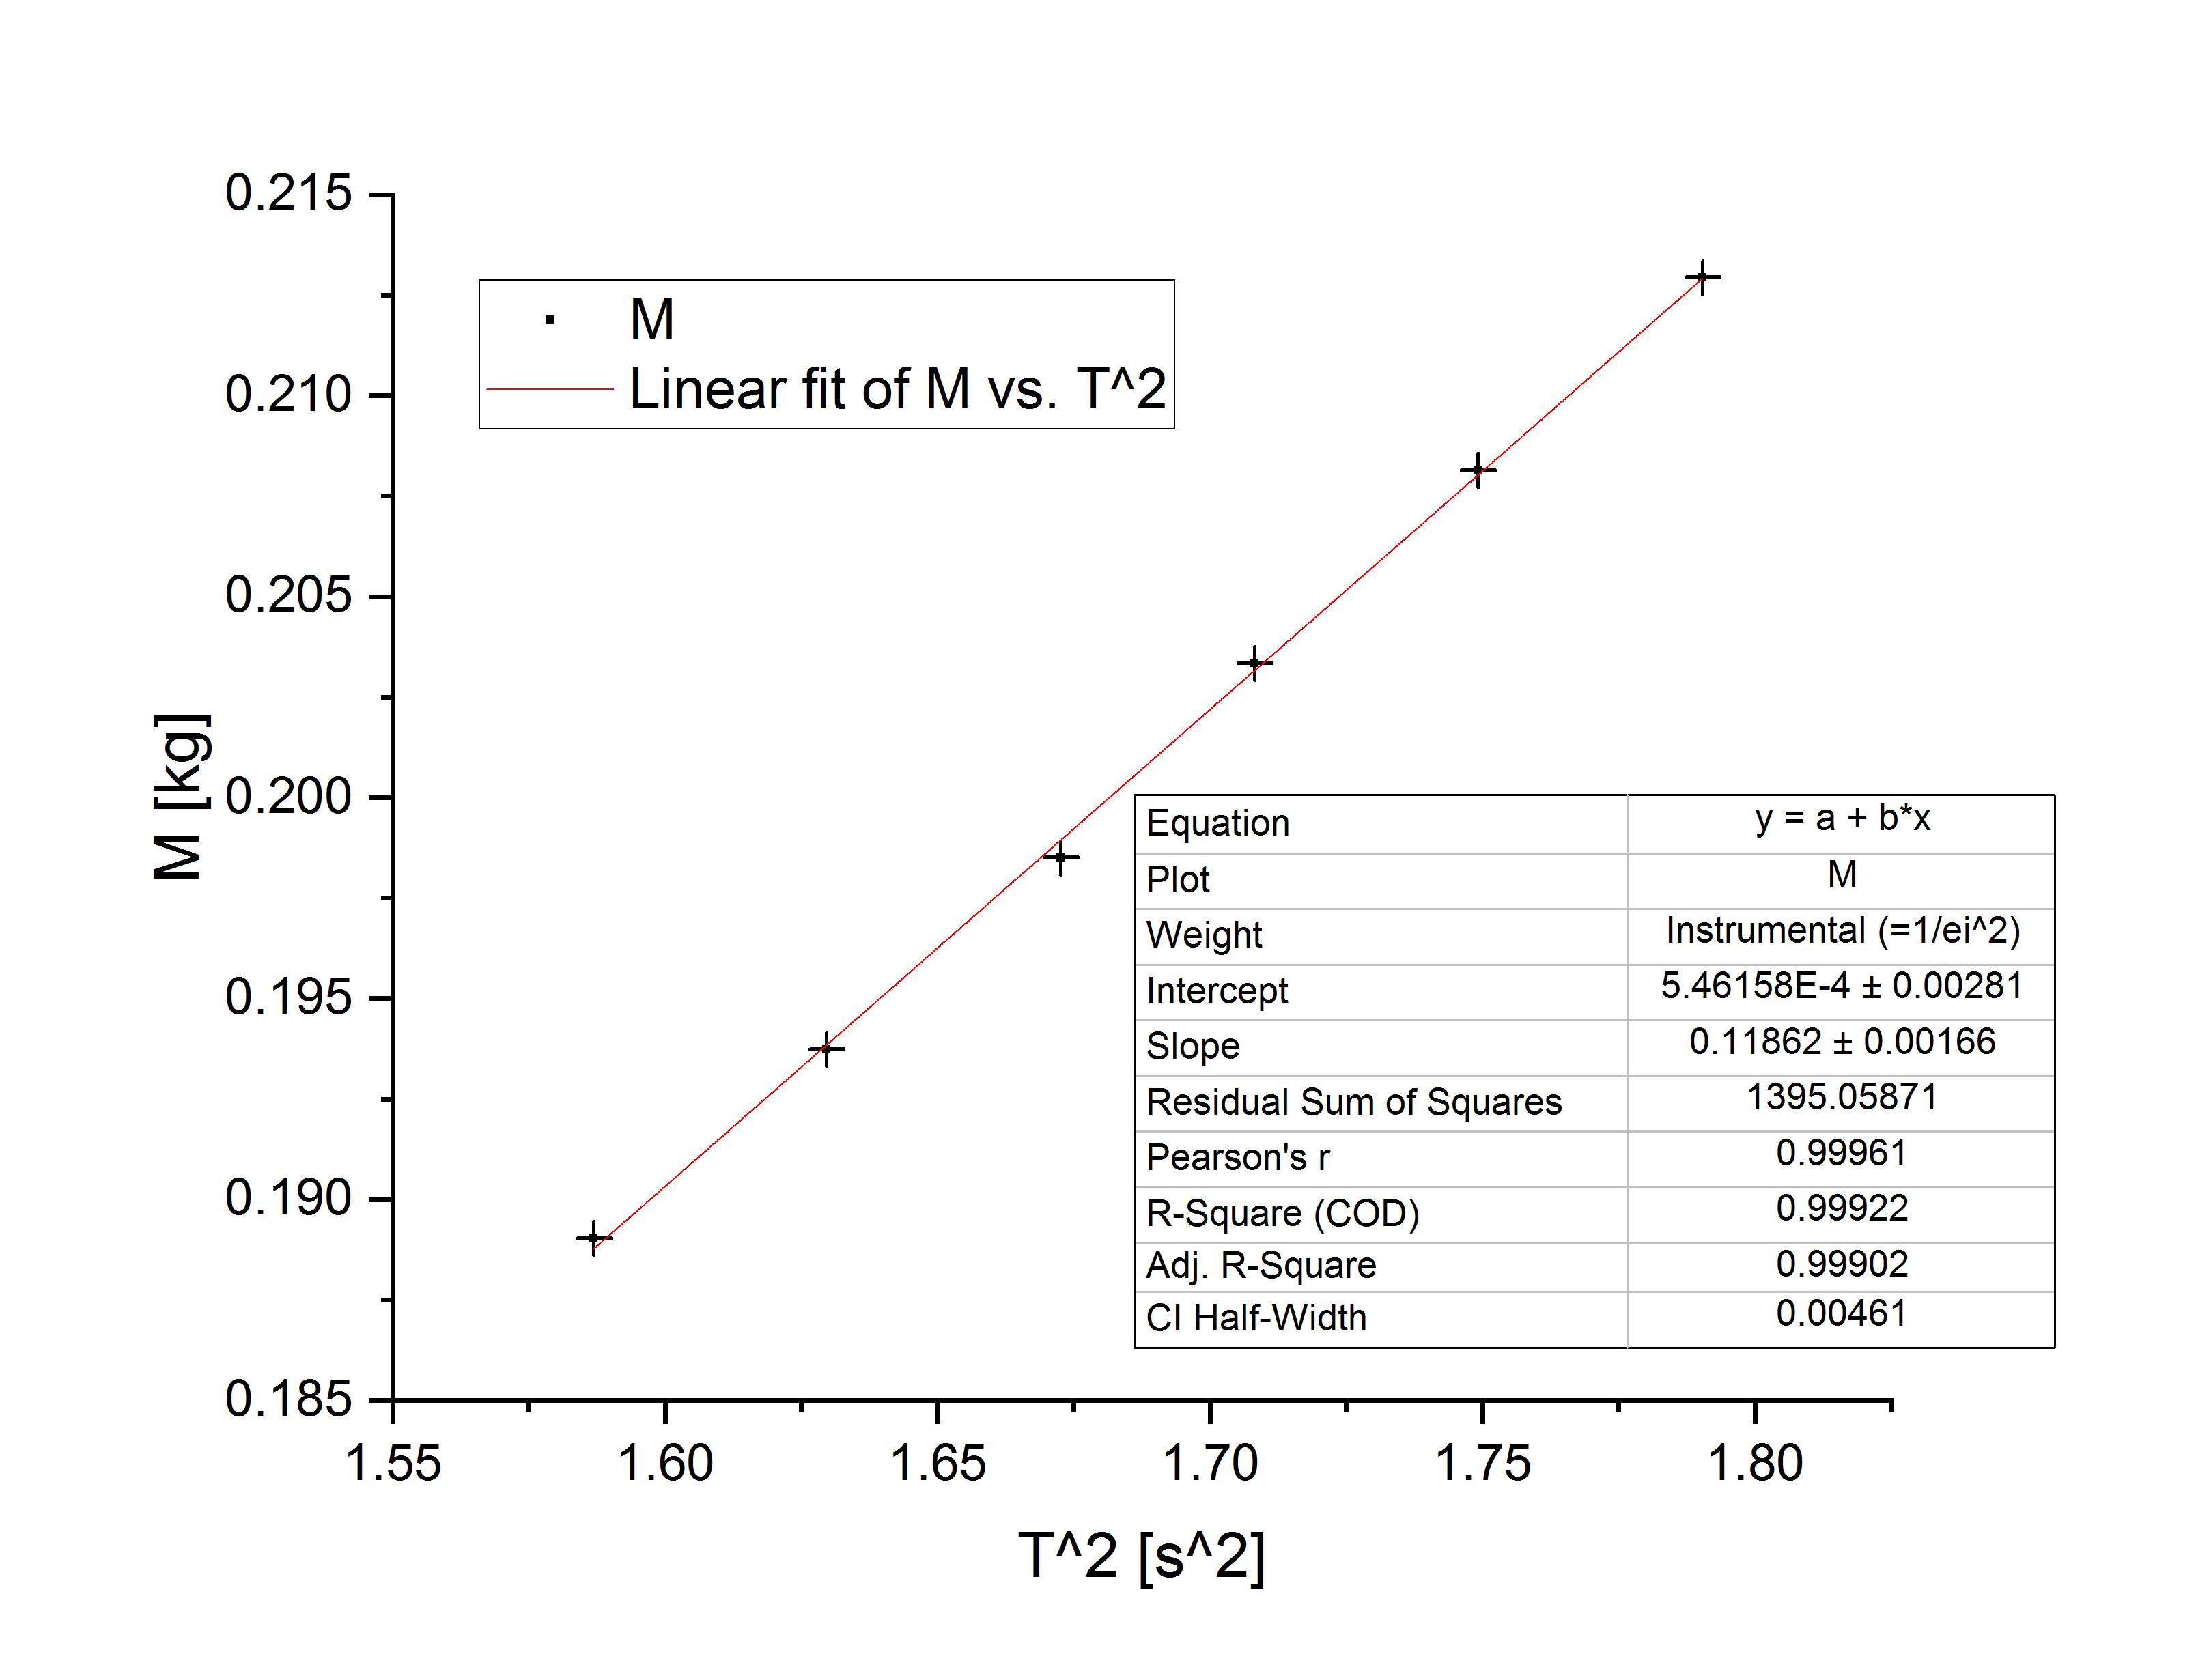
\includegraphics[width=1\textwidth]{pic5} 
    \caption{Linear Fit of $M$ vs. $T^2$ (incline 1).} 
\end{figure}

\begin{figure}[p] 
    \centering
    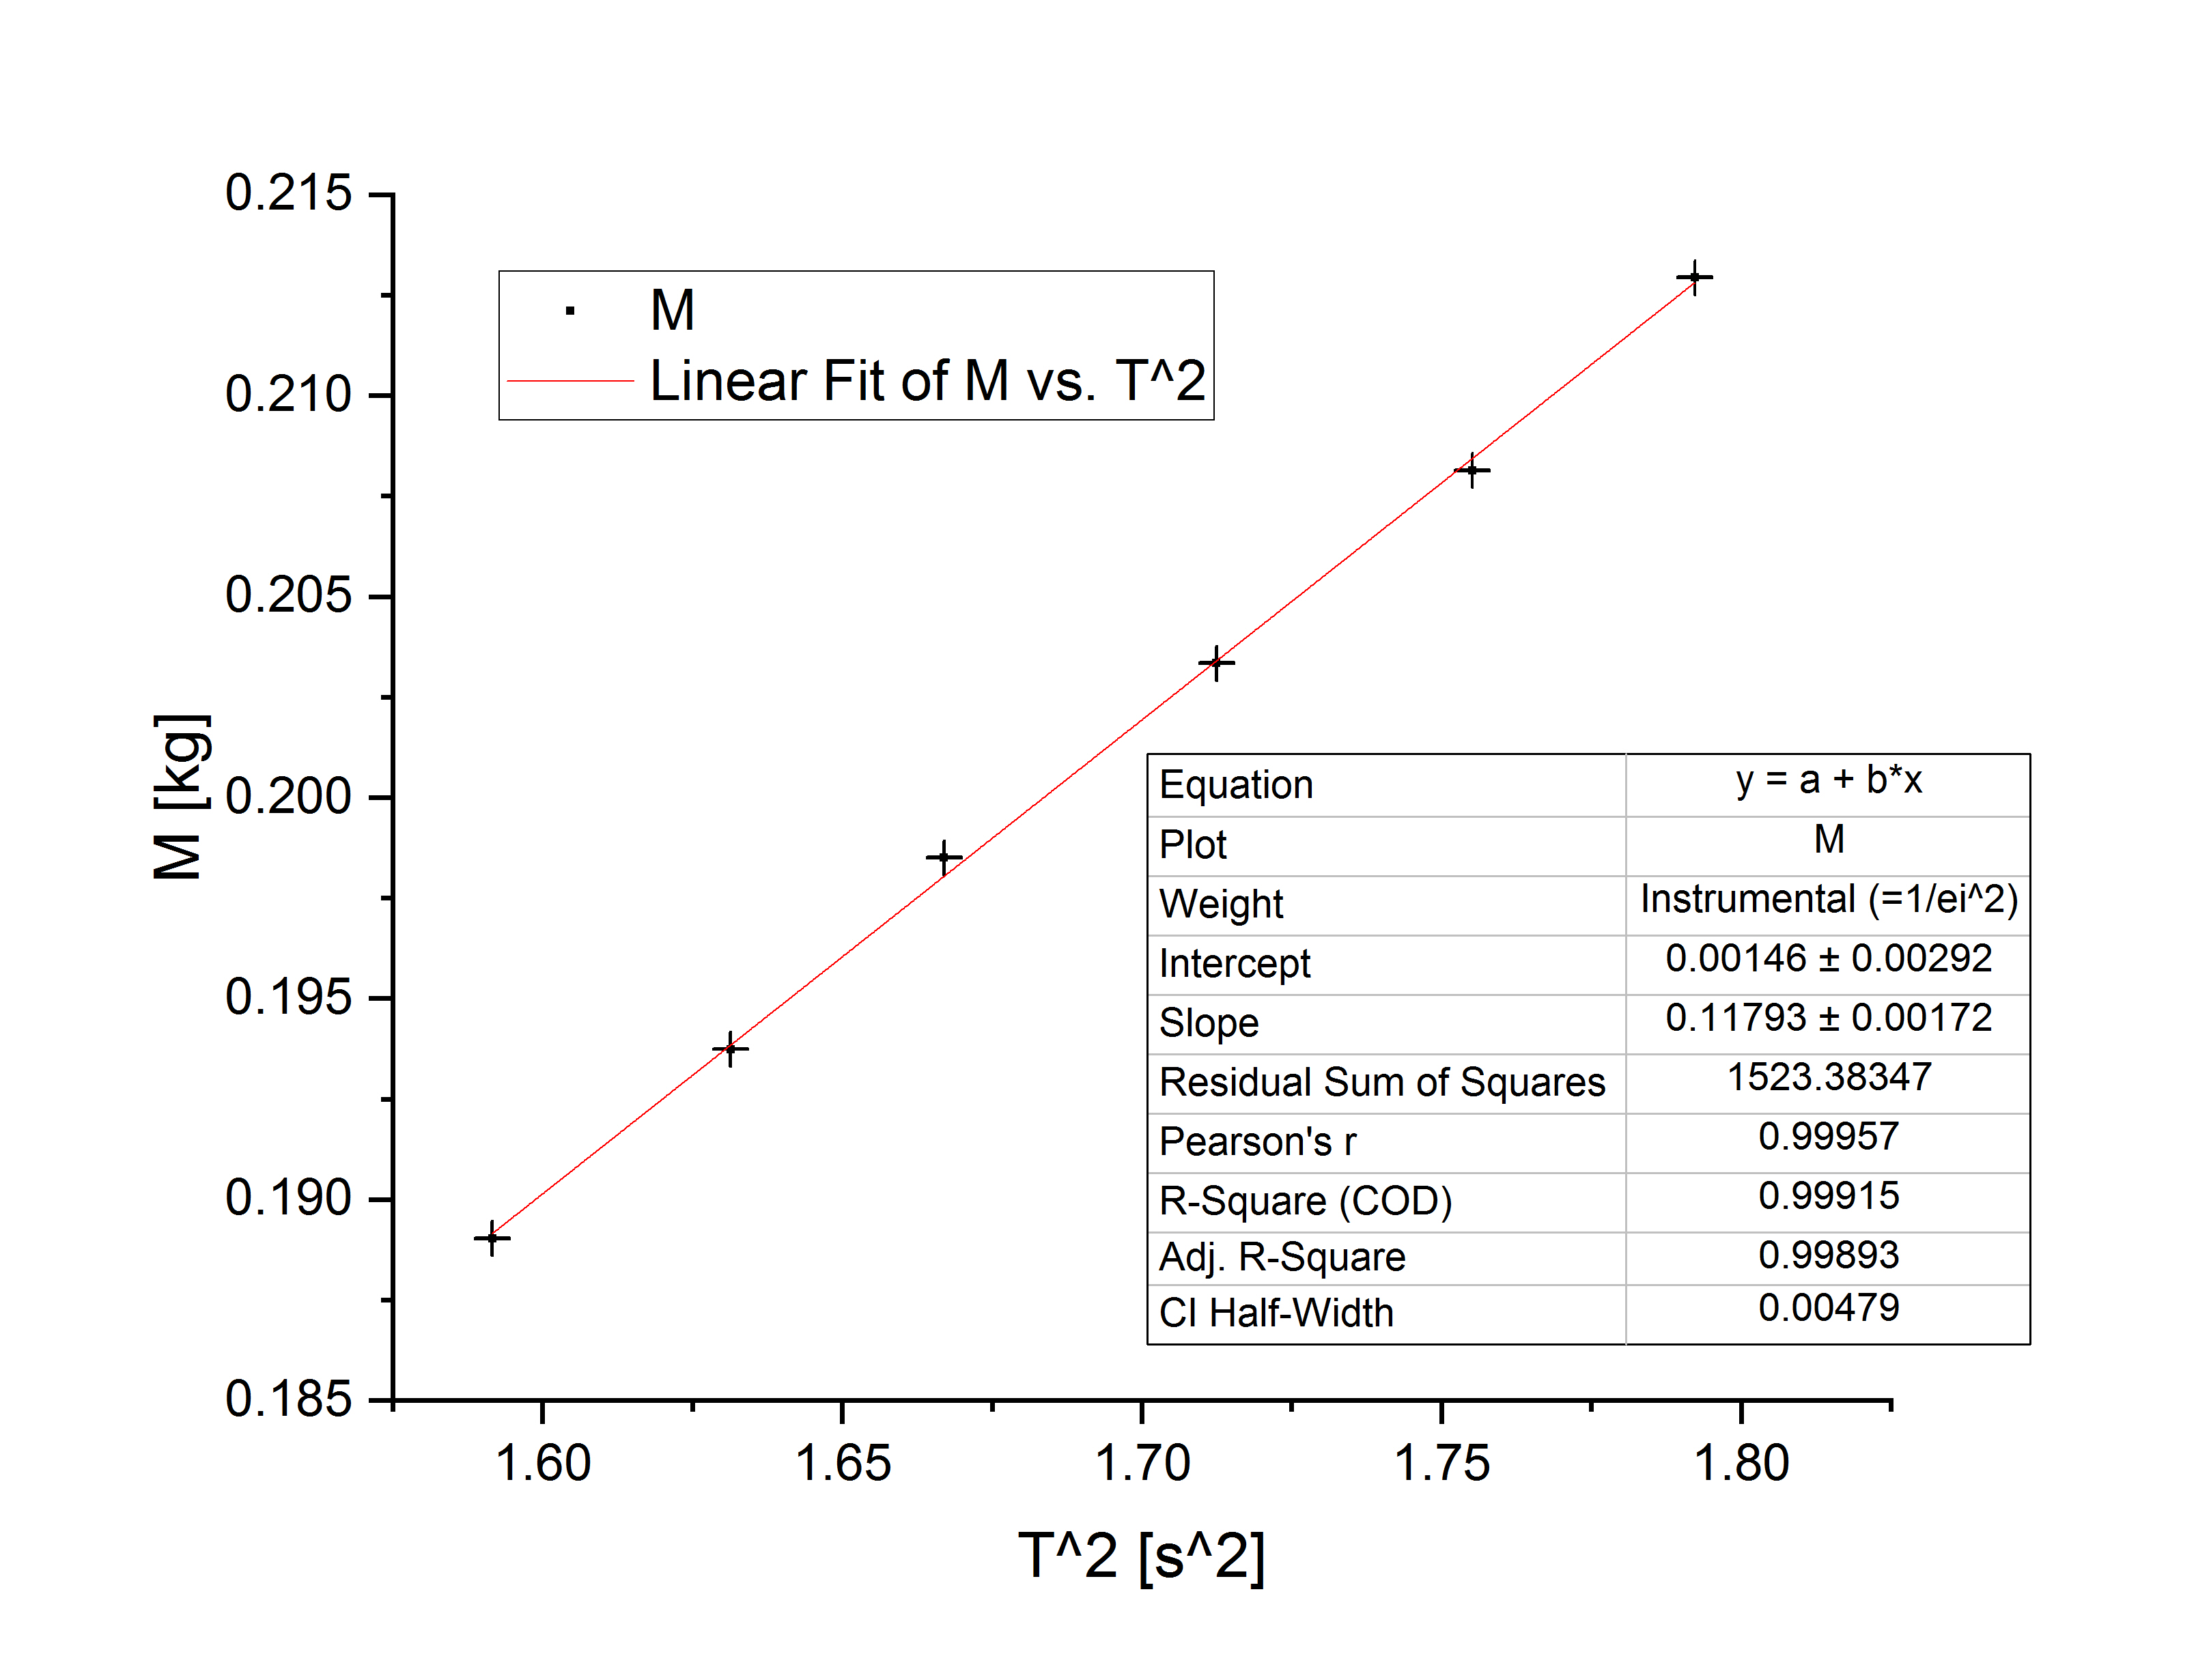
\includegraphics[width=1\textwidth]{pic6} 
    \caption{Linear Fit of $M$ vs. $T^2$ (incline 2).} 
\end{figure}

\par From Eq.(7), we obtain that
\begin{center}
$\displaystyle M = \frac{k}{4\pi^2} T^2$
\end{center}
where $k$ is our spring constant.
\par From the three graphs, we obtain their slopes and corresponding relative uncertainties as follows:
\begin{center}
$ k_{slope, h} = 0.129 [N/m] \pm 0.006 [N/m]$ ~~~~~~ $ u_h = 5\% $
\end{center}
\begin{center}
$ k_{slope, i1} = 0.119 [N/m] \pm 0.005 [N/m]$ ~~~~~~ $ u_h = 4\% $
\end{center}
\begin{center}
$ k_{slope, i2} = 0.118 [N/m] \pm 0.005 [N/m]$ ~~~~~~ $ u_h = 4\% $
\end{center}
\par Because $ k = 4\pi^2 k_{slope} $, we can further find out the spring constants respectively:
\begin{center}
$ k_{h} = 5.1 [N/m] \pm 0.2 [N/m]$ ~~~~~~ $ u_h = 5\% $
\end{center}
\begin{center}
$ k_{i1} = 4.68 [N/m] \pm 0.18 [N/m]$ ~~~~~~ $ u_h = 4\% $
\end{center}
\begin{center}
$ k_{i2} = 4.66 [N/m] \pm 0.19 [N/m]$ ~~~~~~ $ u_h = 4\% $
\end{center}
\par In conclusion, it can be find the following formula is satisfied 
\begin{center}
$ k = k_1 + k_2 $
\end{center}
This will be discussed later in Discussion.

\subsection{\textsc{Relation Between the Oscillation Period T and the Amplitude A}}
In this section, we focus on the relationship between oscillation period $T$ and amplitude $A$. The data are recorded in Table 12.

\begin{table}[h]
\begin{center}
\begin{tabular}{|c|c|c|}
\hline
\multicolumn{2}{|c|}{A[cm] $\pm$ 0.1[cm]} & ten periods [s] $\pm$ 0.0001 [s] \\
\hline
1 & 5.0 & 13.3788 \\
2 & 10.0 & 13.3800 \\
3 & 15.0 & 13.3884 \\
4 & 20.0 & 13.3930 \\
5 & 25.0 & 13.3929 \\
6 & 30.0 & 13.3940 \\
\hline
\end{tabular}
\end{center}
\caption{Data for T vs. A relation.}
\end{table}

\par In this section, we plan to plot a T vs. A linear fit. Hence we ought to find out these two parameters' uncertainties. First, we focus on the period $T$. Since the formula is given by
\begin{center}
$\displaystyle T_i = \frac{T_{10,i}}{10} $
\end{center}
we are able to find out its uncertainty (The detailed calculations are shown in A.4):
\begin{center}
$\displaystyle u_{T_i} = \sqrt{(\frac{\partial T_i}{\partial T_{10,i}})^2(u_{T_{10,i}})^2} = 0.000010 [s]$
\end{center}
\par Hence, all data and their uncertainties are shown in Table 13.

\begin{table}[p]
\begin{center}
\begin{tabular}{|c|c|c||c|c|c|}
\hline
A[m] & $u_A$ [m] & $ u_{rA} $ & T [s] & $u_T$ [s] & $u_{rT}$ \\
\hline
0.050 & 0.001 & 2\% & 1.337880 & 0.000010 & 0.0007\%\\
0.100 & 0.001 & 1\% & 1.338000 & 0.000010 & 0.0007\%\\
0.150 & 0.001 & 0.7\% & 1.338840 & 0.000010 & 0.0007\%\\
0.200 & 0.001 & 0.5\% & 1.339300 & 0.000010 & 0.0007\%\\
0.250 & 0.001 & 0.4\% & 1.339290 & 0.000010 & 0.0007\%\\
0.300 & 0.001 & 0.3\% & 1.339400 & 0.000010 & 0.0007\%\\
\hline
\end{tabular}
\end{center}
\caption{Uncertainties of T vs. A relation.}
\end{table}
\par Based on the data in Table 13, we are able to use \textit{Origin} to plot a linear fit. The results are shown below (Figure 11).

\begin{figure}[p] 
    \centering
    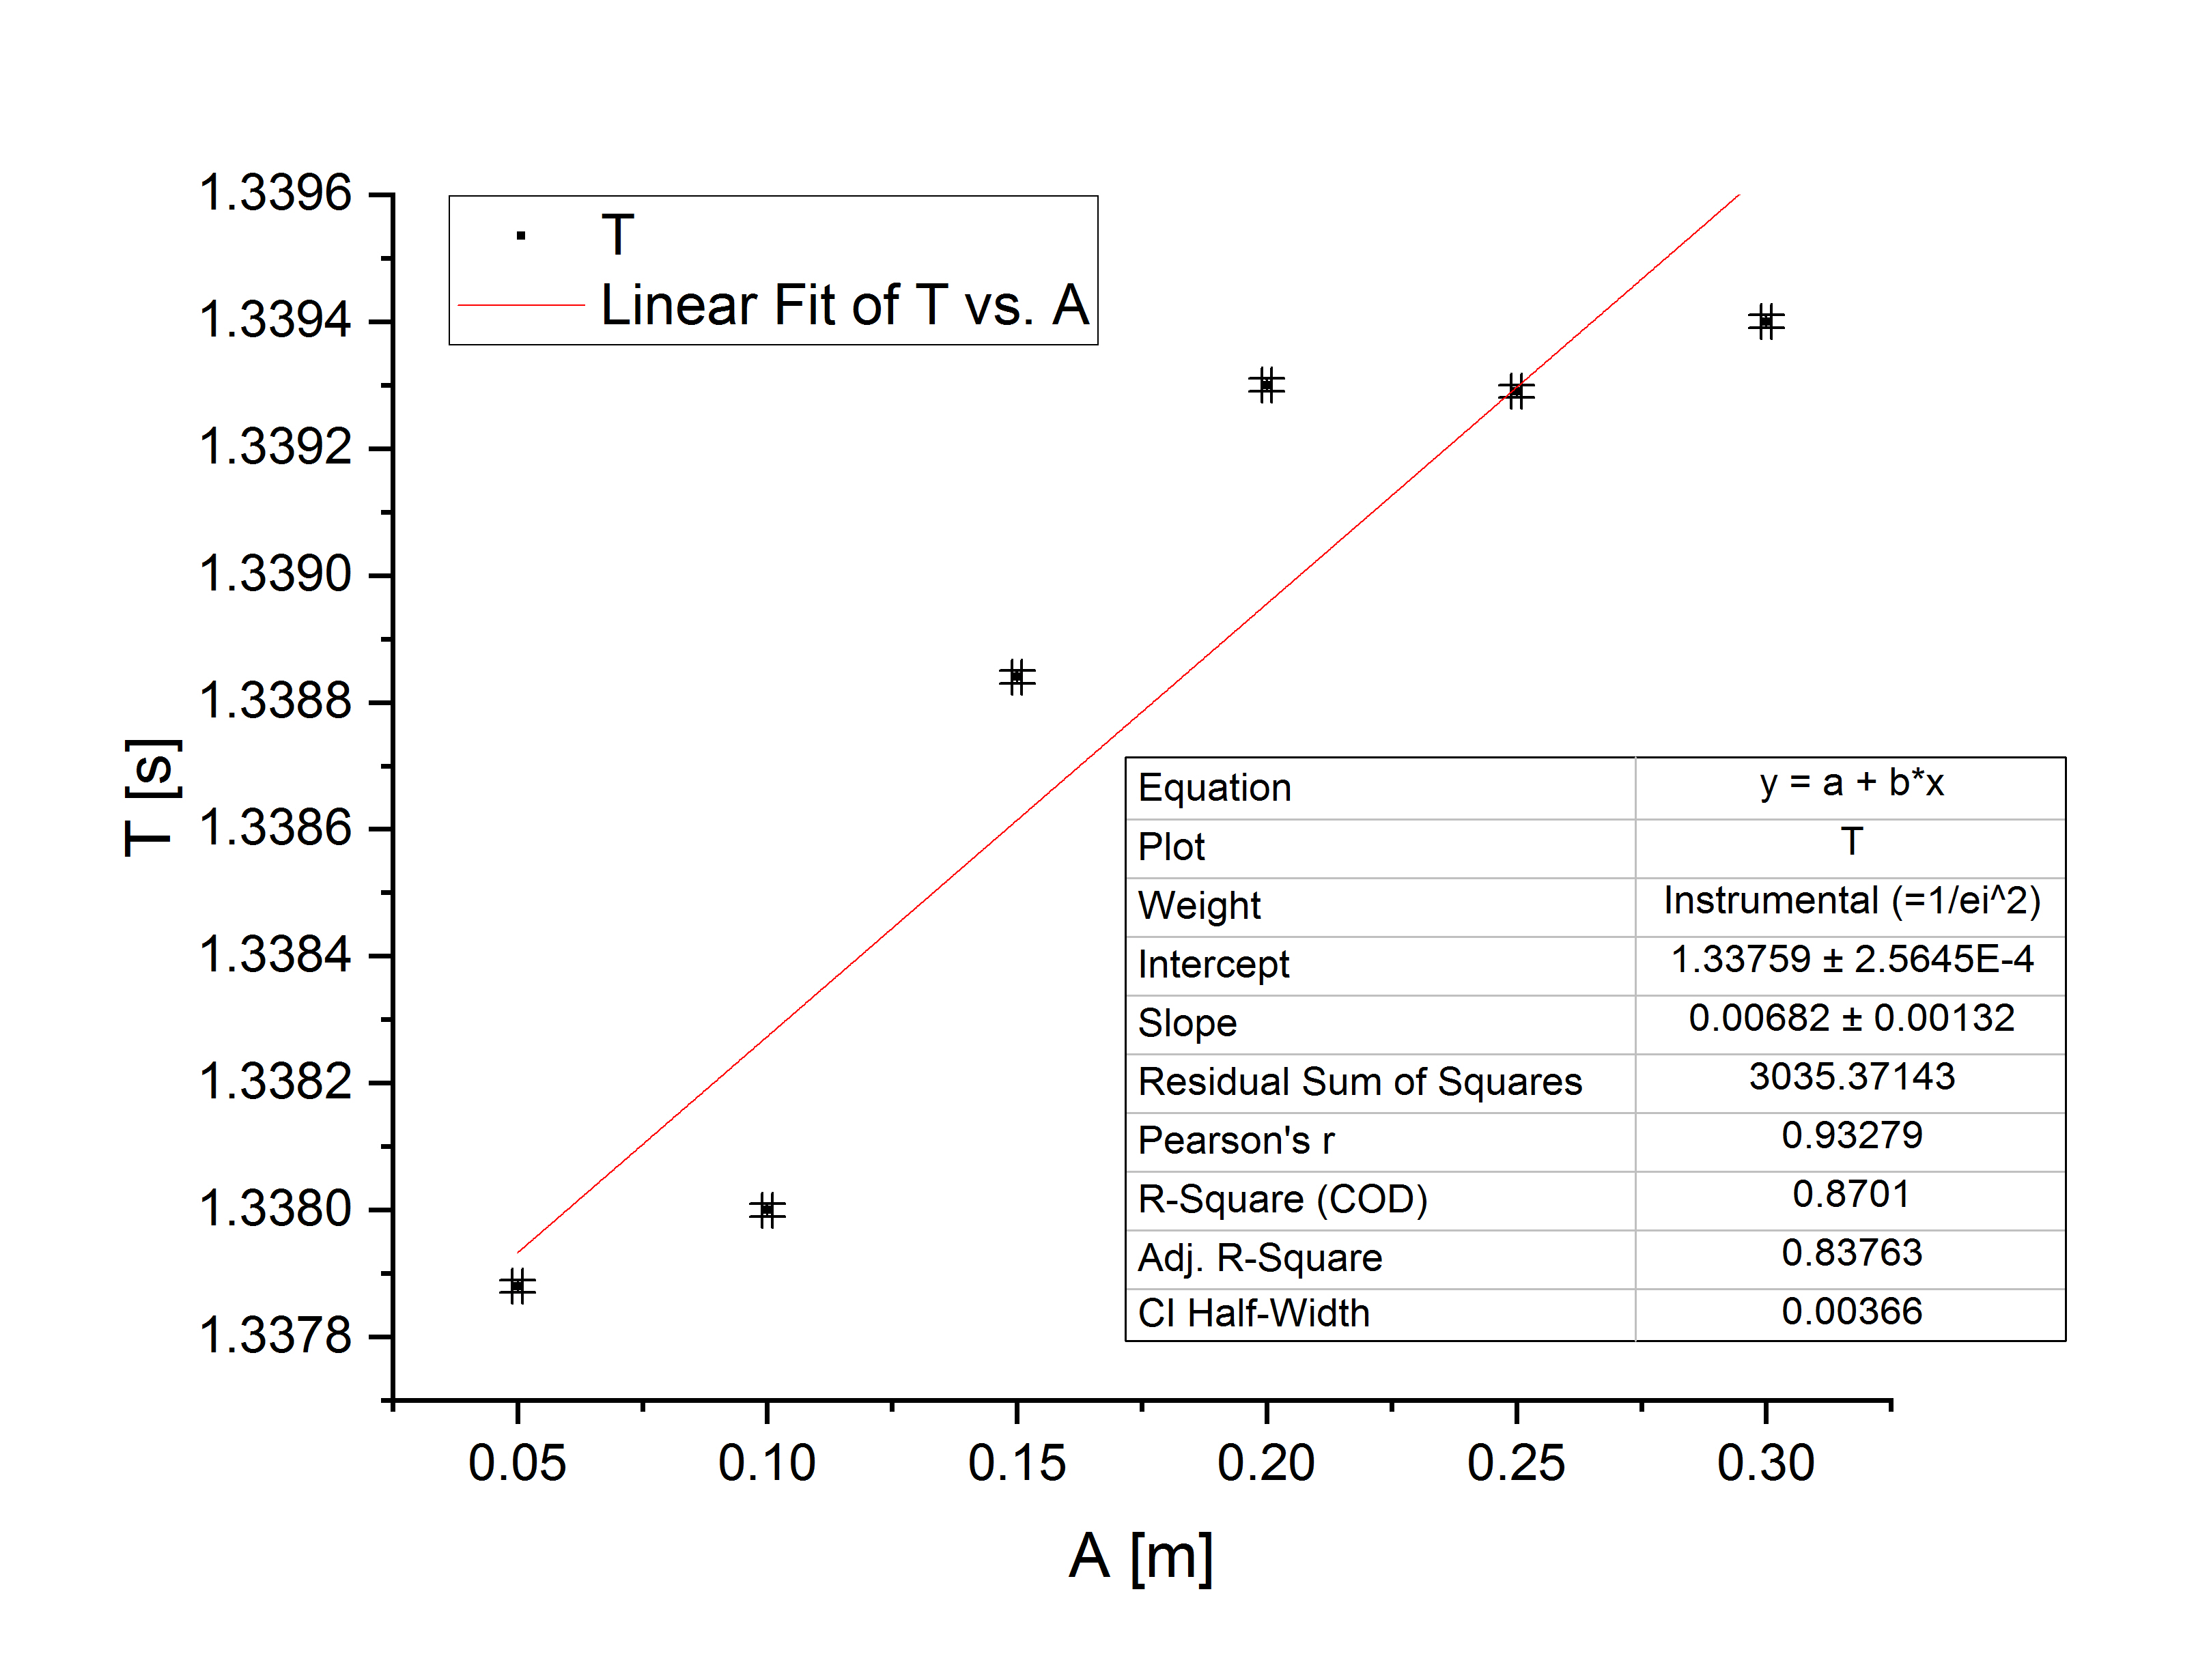
\includegraphics[width=1\textwidth]{pic7} 
    \caption{Linear Fit of $T$ vs. $A$.} 
\end{figure}

\par From the linear fit plot, we obtain the correlation coefficient $\gamma$ and its uncertainty as follows:
\begin{center}
$ \gamma = 0.007 \pm 0.004 $ ~~~~~~ $u_{r\gamma} = 57\%$
\end{center}
\par In this linear fit, the Pearson's r is 0.9. According to the linear dependence, since the Pearson' r is larger than 0.75, then there possibly exist a linear relation between $T$ and $A$. However, theoretically speaking, it is obvious that there is no relationship between $T$ and $A$. What leads to the contradiction will be discussed later.

\subsection{\textsc{Relation Between the Maximum Speed and the Amplitude}}
In this section, we study the relation between the maximum speed and amplitude. First, the measurement data are recorded in Table 14 and Table 15.

\begin{table}[h]
\begin{center}
\begin{tabular}{|c|c|c|}
\hline
\multicolumn{2}{|c|}{A[cm] $\pm$ 0.1[cm]} & $\Delta t$ [s] $\pm$ 0.00001 [s] \\
\hline
1 & 5.0 & 0.04244 \\
2 & 10.0 & 0.02154 \\
3 & 15.0 & 0.01411 \\
4 & 20.0 & 0.01058 \\
5 & 25.0 & 0.00848 \\
6 & 30.0 & 0.00707 \\
\hline
\end{tabular}
\end{center}
\caption{Data for the $v_{max}^2$ vs. $A^2$ relation.}
\end{table}

\begin{table}[h]
\begin{center}
\begin{tabular}{|c|c|}
\hline
$x_{in}$ [mm] $\pm$ 0.02 [mm] & $x_{out}$ [mm] $\pm$ 0.02 [mm] \\
\hline
4.50 & 15.42 \\
4.50 & 15.42 \\
4.50 & 15.42 \\
\hline
\end{tabular}
\end{center}
\caption{Data for the $v_{max}^2$ vs. $A^2$ relation.}
\end{table}

\newpage
Then, we first try to figure out $v$. To achieve this, we calculate the distance between two blanks on the U-shape shutter, i.e., we have (The detailed calculations are shown in Appendix A.5.)
\begin{center}
$\displaystyle x_{in} = \frac{\sum_{i=1}^3x_{in,i}}{3} = 0.00450 [m] \pm 0.00002 [m]$ ~~~~~~$ u_{rin} = 0.4\% $
\end{center}
\begin{center}
$\displaystyle x_{out} = \frac{\sum_{i=1}^3x_{out,i}}{3} = 0.01542 [m] \pm 0.00002 [m] ~~~~~~ u_{rout} = 0.13\% $
\end{center}

\par After that, we can have
\begin{center}
$\displaystyle \Delta x = \frac{x_{in} + x_{out}}{2} = 9.960 [mm] \pm 0.014 [mm] = 0.009960 [m] \pm 0.000014[m]$
\end{center}
with a relative uncertainty 
\begin{center}
$\displaystyle u_{r\Delta_x} = 0.14\%$
\end{center}
Now, we would like to find out $Mv_{max}^2$, which is given by
\begin{center}
$\displaystyle Mv_{max}^2 = M(\frac{\Delta x}{\Delta t})^2$
\end{center}
And $A^2$ similarly.
\par The detailed calculation are shown in Appendix A.5, and the final data with uncertainties are shown in Table 16.

\begin{table}[h]
\begin{center}
\begin{tabular}{|c|c|c||c|c|c|}
\hline
$ Mv_{max}^2 $ [J] & $u_{Mv_{max}^2}$ [J] & $u_{rMv_{max}^2}$ & $A^2 [m^2]$ & $ u_{A^2} $ & $ u_{rA^2}$ \\
\hline
0.01086 & 0.00003 &  0.3\%  & 0.00250 & 0.00010 & 4\%\\
0.04216 & 0.00013 &  0.3\%  & 0.0100 & 0.0002 & 2\%\\
0.0982 & 0.0003 &  0.3\%  & 0.0225 & 0.0003 & 1.3\%\\
0.1747 & 0.0006 &  0.3\%  & 0.0400 & 0.0004 & 1\%\\
0.2720 & 0.0011 &  0.4\%  & 0.0625 & 0.0005 & 0.8\%\\
0.3913 & 0.0018 &  0.5\%  & 0.0900 & 0.0006 & 0.7\%\\
\hline
\end{tabular}
\end{center}
\caption{Uncertainties for the $v_{max}^2$ vs. $A^2$ relation.}
\end{table}

\par Now, we can use \textit{Origin} to plot a linear fit. The figure is shown in Figure 12.
\par From Eq.(12), we know that 
\begin{center}
$k A^2 = mv_{max}^2$
\end{center}
Because the system is connected in parallel, the spring constant $k$ is supposed to be the sum of the two springs $k_1 + k_2$. Namely, we have
\begin{center}
$ Mv_{max}^2 = (k_1 + k_2)A^2 $
\end{center}
where $k_1+k_2$ is the slope of the linear fit.

\begin{figure}[p] 
    \centering
    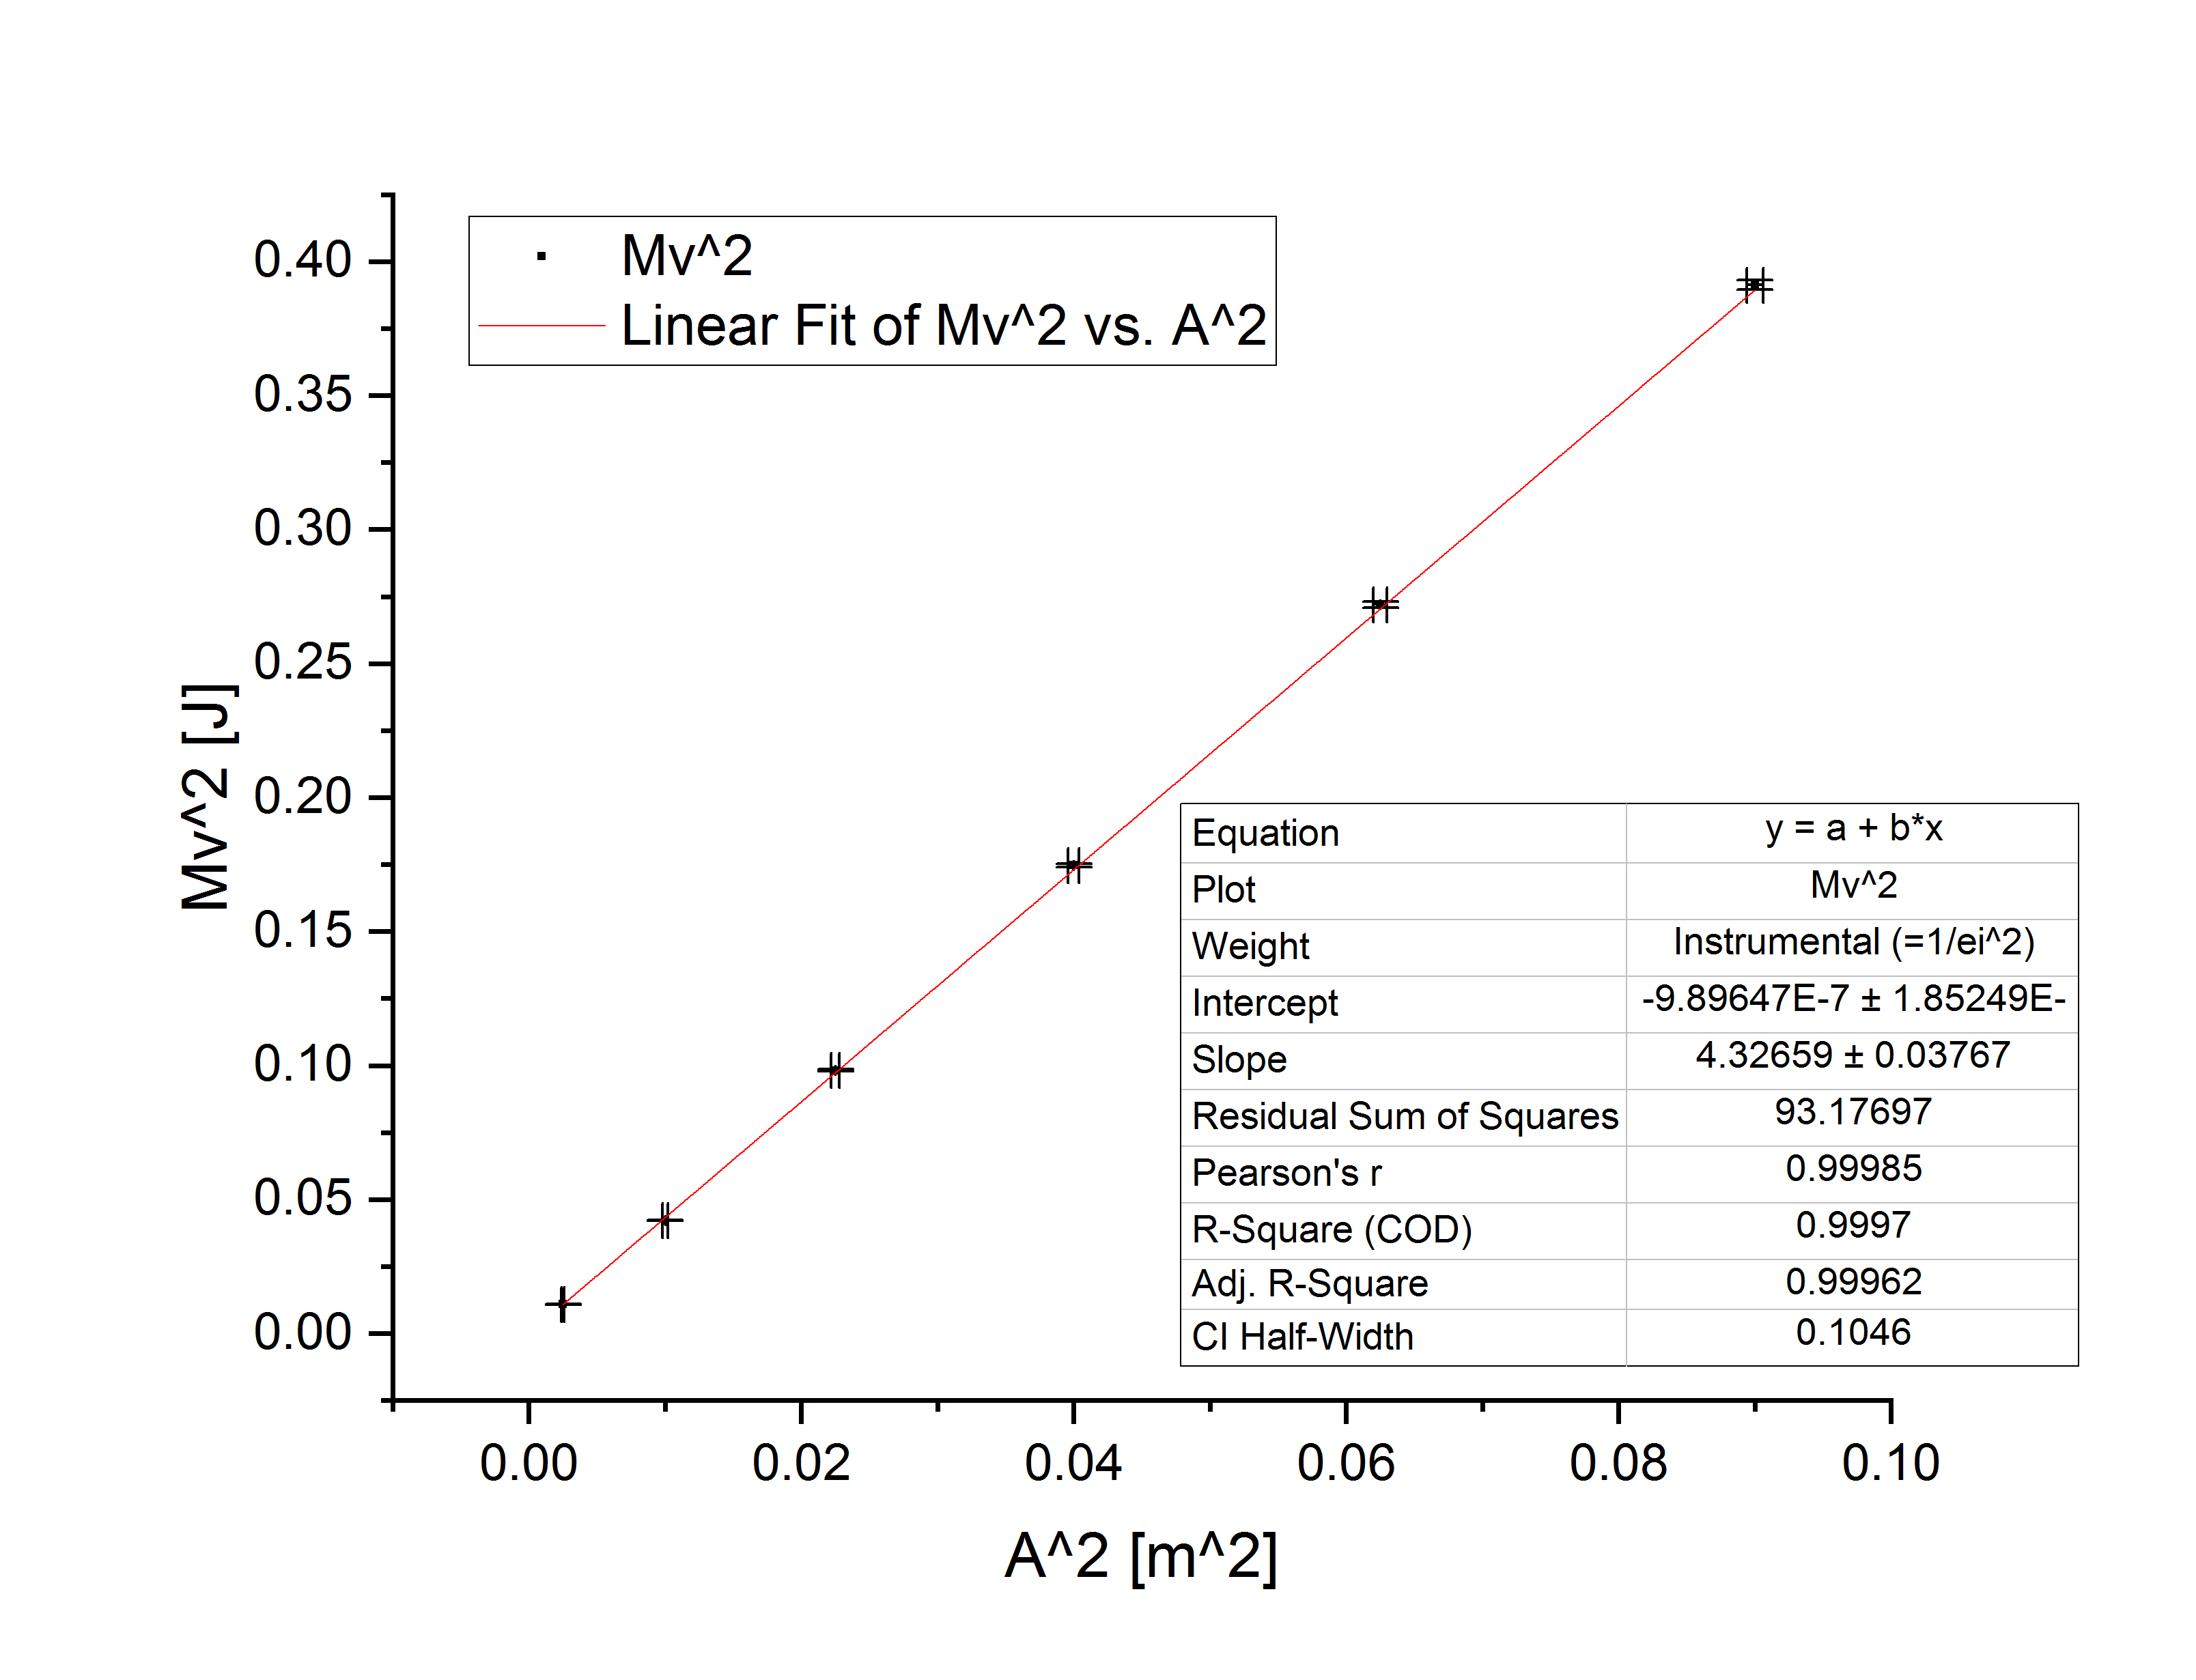
\includegraphics[width=1\textwidth]{pic8} 
    \caption{Linear Fit of $M^2$ vs. $A^2$.} 
\end{figure}

\par Hence, from Figure 12, we obtain the slope and uncertainty of the linear fit is:
\begin{center}
$ k_v = 4.33 [N/m] \pm 0.10 [N/m] $ ~~~~~~ $ u_{rk_v} = 2\% $
\end{center}

In 4.2 we have already figured out the spring constant $k_1 = 2.17 [N/m] $ and $k_2 = 2.47[N/m]$. Therefore, the theoretical value of the slope is 
\begin{center}
$k_p = k_1 + k_2 = 4.64 [N/m] \pm 0.12 [N/m] $ ~~~~~~ $ u_{rk_p} = 3\% $
\end{center}

\par We compare the theoretical value with the measured one, and then calculate the deviation from the theoretical value:
\begin{center}
$\displaystyle d = \frac{|k_v - k_p|}{k_p} \times 100\% = 7\% $
\end{center}

%----------------------------------------------------------------------------------------
%	SECTION 5
%----------------------------------------------------------------------------------------
\newpage
\section{\textsc{Discussion}}
\subsection{\textsc{The spring constant}}
\subsubsection{\textsc{Springs in series}}
In this lab, we use the Jolly balance to measure the spring constant of the spring and verify the theorem of springs in series. The value we obtain in our experiment are recorded below:
\begin{center}
$ k_1 = 2.17 [N/m] \pm 0.03 [N/m] $ ~~~~~~ $ u_{k1} = 1.4\% $
\end{center}
\begin{center}
$ k_2 = 2.47 [N/m] \pm 0.09 [N/m] $ ~~~~~~ $ u_{k2} = 4\% $
\end{center}
\begin{center}
$ k_s = 1.162[N/m] \pm 0.008[N/m] $ ~~~~~~ $ u_{ks} = 0.7\% $
\end{center}
\par Then, we calculate the theoretical value of the springs in series and compare it with our measured value. The result has been shown below:
\begin{center}
$\displaystyle  k_{th} = \frac{k_1k_2}{k_1+k_2} = 1.16 [N/m] \pm 0.02 [N/m]$ ~~~~~~ $ u_{rk_{th}} = 2\% $
\end{center}
\par Now, we are able to calculate the deviation of the experimental value between the measured value as follows:
\begin{center}
$ \displaystyle u_{r} = \frac{|k_{th} - k_s|}{k_{th}}\times 100\% = 0.17 \% $
\end{center}
In this way, we can conclude that our result is reliable and our experiment is successful in general. The satisfactory result may comes from:
\begin{itemize}
\item The high precision of the Jolly balance.
\item The load is not too large so that the springs are in their elastic limit. 
\item The accurate performance of the procedure.
\end{itemize}
\subsubsection{\textsc{Springs in parallel}}
In this lab, we also verify the situation where the springs are connected parallel. This is realized by studying the cart on an air track. The technical details have been shown in 4.5, and our result are shown below:
\begin{center}
$ k_v = 4.33 [N/m] \pm 0.10 [N/m] $ ~~~~~~ $ u_{rk_v} = 2\% $
\end{center}

\par Then, we find out the theoretical value of the slope:
\begin{center}
$k_p = k_1 + k_2 = 4.64 [N/m] \pm 0.12 [N/m] $ ~~~~~~ $ u_{rk_p} = 3\% $
\end{center}
\par We compare the theoretical value with the measured one, and then calculate the deviation from the theoretical value:
\begin{center}
$\displaystyle d = \frac{|k_v - k_p|}{k_p} \times 100\% = 7\% $
\end{center}
\par Unfortunately, the deviation reaches $7\%$, which is relatively high compared with the $0.17\%$ in 5.1.1. There may be a variety of reasons which may lead to this large difference:
\begin{itemize}
\item Although we have used the air track to minimize the friction, there still exist some small friction between the contact surfaces, whose influence can not be neglected with the increase of oscillation amplitude. For instance, when $A = \pm 30 [cm]$, the influence of friction can't be easily neglected.
\item In the lab, there also exists air drag, which can not be ignored when the velocity of the cart becomes large. To be more specific, when doing the experiment, we found that when the amplitude is set to be $A = \pm 30[cm]$, it will decrease to approximately $25[cm]$ after 10 periods of oscillation. This means that the existence of air drag and friction can't be ignored in this case.
\item Because in this lab, we stretch the springs to as long as $30 [cm]$ to obtain our data, chances are that the deformation exceeds its elastic limit, and the irreversible deformation of springs is sure to make some deviations.
\item The air track may not be completely horizontal, and the small inclination may lead to some subtle difference on environment, which will influence the result.
\end{itemize}
\subsection{\textsc{Relation Between the Oscillation Period T and the Mass of the Oscillator M}}
In this section, we apply an $M$ vs. $T^2$ linear fit, and we find out that our Pearson's r is close to 1:
\begin{center}
$ r = 0.99939 \approx 1 $
\end{center}
Since the r is larger than 0.75, it is possibly that there exist a linear relation between $M$ and $T^2$. From our theoretical analysis, the slope is:
\begin{center}
$ \displaystyle k_{slope} = \frac{k}{4\pi^2} $
\end{center}
\par Thus, we have
\begin{center}
$ k_{h} = 5.1 [N/m] \pm 0.2 [N/m]$ ~~~~~~ $ u_h = 5\% $
\end{center}
\begin{center}
$ k_{i1} = 4.68 [N/m] \pm 0.18 [N/m]$ ~~~~~~ $ u_h = 4\% $
\end{center}
\begin{center}
$ k_{i2} = 4.66 [N/m] \pm 0.19 [N/m]$ ~~~~~~ $ u_h = 4\% $
\end{center}
\par In conclusion, it can be find the following formula is satisfied 
\begin{center}
$ k = k_1 + k_2 $
\end{center}
It can be noticed that our first result has a large difference from the other two ones. And some reason may lead to such difference:
\begin{itemize}
\item The I-shape shutter contact the sensor when moving back and through, which leads to error in time recording.
\item The air track may not be that horizontal, which may lead to errors.
\end{itemize}
\subsection{\textsc{Relation Between the Oscillation Period T and the Amplitude A}}
In this section, we apply a $T$ vs. $A$ linear fit, and try to find out the relationship between them. The Pearson's r of the linear fit is: 
\begin{center}
$ r = 0.93279 \approx 0.9 $
\end{center}
Since r is larger than 0.75, the result yields a possible relationship between T and A. Nevertheless, theoretically speaking, such relationship doesn't exist. Hence we list some possible factors contributing to the contradiction:
\begin{itemize}
\item This are just some accidental errors. It can be observed from the figure that the points are actually kind of scatter, and chances are that they coincide to have a "linear relation". In other words, it is the accidental errors which lead to the large value of Pearson's r.
\item The friction between the contact surface and the air drag. These factors also influence the result. Since we have discussed them before, we do not discuss then in detail here.
\end{itemize}
\subsection{\textsc{Relation Between the Maximum Speed and the Amplitude}}
In this section, we focus on the relation between the maximum speed and the amplitude, and plot a $Mv_{max}^2$ vs. $A^2$ linear fit. The Pearson's r is:
\begin{center}
$r = 0.9985 \approx 1 $
\end{center}
Since r is larger than 0.75, we can hopefully conclude that there exist a linear relation between $Mv_{max}^2$ and $A^2$. In fact, from our analysis, the slope is just the spring constant.
\subsection{\textsc{Some possible improvement to the experiment}}
Here are some improvement which may increase the accuracy of this experiment:
\begin{itemize}
\item In this lab, the amplitude of the oscillation is hard to control. It's difficult for us to control the amplitude accurately simply by hands or ruler. Hence some improvements may exist here.
\item The number of periods should be carefully chosen. It can neither be too large nor be too small. Too large number of periods may lead to the obvious influence of friction and air drag, while too small number of periods may lead to the instability of data. In our lab, we just choose the number of periods to be 10. However, if the speed of the cart is large, we may decrease the number of periods we measure so that the accuracy is increased.
\item The I-shaped and U-shaped shutter may be unstable in our experiment. To be more specific, it may hit the sensor, or contact the sensor, both of which lead to errors. Hence it would be better if the shutters are much more stable.
\end{itemize}

\section{\textsc{Conclusion}}
In conclusion, in this lab, we have learned a lot:
\begin{itemize}
\item How to use the Jolly balance.
\item How to use \textit{Origin} to plot a linear fit.
\item How to analyse the data involved in a linear fit in terms of Pearson's r. 
\item The factors which may influence the simple harmonic oscillation. 
\end{itemize}
\par Also, we verify some important conclusions:
\begin{itemize}
\item When springs are connected in series, the spring constant satisfies $\displaystyle k = \frac{k_1k_2}{k_1+k_2} $.
\item When springs are connected in parallel, the spring constant satisfies $\displaystyle k = k_1 + k_2 $.
\item Though two quantities do not have a linear relation theoretically, a linear fit may still yield an $r > 0.75$ such that a relation may exist. However, this may simply result from accidental errors.
\item The energy conservation in simple harmonic motion.
\end{itemize}
\par In all, in lab 3 I really learned a lot, and my understanding towards simple harmonic motion becomes deeper and deeper. Although some errors may still exist, the factors have been detected and hopefully we have successfully accomplished this experiment.
%----------------------------------------------------------------------------------------
%	SECTION 6
%----------------------------------------------------------------------------------------
\newpage

\begin{appendices} 
      \section{\textsc{Measurement uncertainty analysis}} 
      \subsection{\textsc{Uncertainty of mass measurement}}      
      First, we calculate the uncertainty of mass. For other masses except the equivalent mass, since it is a single measurement, the type A uncertainties equal to zero, and the type B uncertainty is 0.01 [g] which is due to the instruments. Hence the overall uncertainty is:
      \begin{center}
      $u = \sqrt{\Delta_A^2 + \Delta_B^2} = 0.001 [g]$
      \end{center}
      For the equivalent mass M, however, the uncertainty propagation should be considered. Since the formula are expressed as follows:
      \begin{center}
      $ \displaystyle M_I = m_I + \frac{1}{3}m_{spr1,2} $
      \end{center}
      \begin{center}
      $ \displaystyle M_U = m_U + \frac{1}{3}m_{spr1,2} $
      \end{center}
      The uncertainty can be calculated as follows:
      \begin{center}
      $ \displaystyle \frac{\partial M_I}{\partial{m_I}} = 1 $
      \end{center}
       \begin{center}
      $ \displaystyle \frac{\partial M_I}{\partial{m_{spr1,2}}} = \frac{1}{3} $
      \end{center}
      Therefore, we obtain:
      \begin{center}
      $ \displaystyle u_{M_I} = \sqrt{(\frac{\partial M_I}{\partial{m_I}})^2(u_{M_I})^2 + (\frac{\partial M_I}{\partial{m_{spr1,2}}})^2(u_{m_{spr1,2}})^2} = 0.011 [g]$
      \end{center}
      Similarly, we have:
      \begin{center}
      $ \displaystyle u_{M_U} = \sqrt{(\frac{\partial M_U}{\partial{m_U}})^2(u_{M_U})^2 + (\frac{\partial M_U}{\partial{m_{spr1,2}}})^2(u_{m_{spr1,2}})^2} = 0.011 [g]$
      \end{center}
      Hence, the equivalent mass with their relative uncertainties can be obtained as follows:
      \begin{center}
      $ \displaystyle M_I = m_I + \frac{1}{3}m_{spr1,2} = 184.327 [g] \pm 0.011 [g] ~~~~~~ u_{rM_I} = 0.006\%$
      \end{center}
      \begin{center}
      $ \displaystyle M_U = m_U + \frac{1}{3}m_{spr1,2} = 192.477 [g] \pm 0.011 [g] ~~~~~~ u_{rM_U} = 0.006\%$
      \end{center}
      \subsection{\textsc{Uncertainty of spring constant}}      
      To find out the spring constant, first we use the Jolly balance, and the uncertainties of the $\Delta L$ are what we should obtain first. Since we only measure the value once, the type A uncertainty for length measurement always equals to 0. Thus the overall uncertainty is simply the type B uncertainty, namely, $u_{L_i} = 0.01 [cm] = 0.0001 [m]$. Furthermore, because the measurement is indirect, the propagation of uncertainty should be considered, and we calculate the partial derivatives first.
      \begin{center}
      $ \Delta L_i = L_i - L_0 $
      \end{center}
      \begin{center}
      $ \displaystyle \frac{\partial \Delta L_i}{\partial L_i} = 1 $
      \end{center}
      \begin{center}
      $ \displaystyle \frac{\partial \Delta L_i}{\partial L_0} = -1 $
      \end{center}
      \begin{center}
      $ \displaystyle u_{\Delta L_i} = \sqrt{(\frac{\partial \Delta L_i}{\partial L_i})^2(u_{L_i})^2 + (\frac{\partial \Delta L_i}{\partial L_0})^2(u_{L_0})^2} = 0.014 [cm] = 0.00014 [m]$
      \end{center}
\par Also, in this section, the weight of the loads and their uncertainties are also needed. Since we have:
	\begin{center}
	$ G = mg $
	\end{center}
we can further obtain that:
	\begin{center}
	$\displaystyle u_G = \sqrt{(\frac{\partial G}{\partial m})^2(u_m)^2} = 0.00010 [N]$
	\end{center}
\par Then, we obtain the uncertainties of the spring constant of 1, 2, and in series with the help of \textit{Origin}, and the value are listed below:
\begin{center}
$ u_{k1} = 0.03 [N/m] $
\end{center}
\begin{center}
$ u_{k2} = 0.09 [N/m] $
\end{center}
\begin{center}
$ u_{ks} = 0.008 [N/m] $
\end{center}
\par Now, we calculate the theoretical value of the spring in series based on $k_1$ and $k_2$. The formula to calculate $k_{th}$ can be expressed as:
\begin{center}
$\displaystyle k_{th} = \frac{k_1k_2}{k_1+k_2} = 1.16 [N/m] \pm 0.02 [N/m]$
\end{center}
\par The uncertainty of $k_{th}$ can be calculate accordingly. First, we write its partial derivatives:
\begin{center}
$ \displaystyle \frac{\partial k_{th}}{\partial k_1} = \frac{k_2^2}{(k_1+k_2)^2} $
\end{center}
\begin{center}
$ \displaystyle \frac{\partial k_{th}}{\partial k_2} = \frac{k_1^2}{(k_1+k_2)^2} $
\end{center}
\par Therefore, the overall uncertainty is:
\begin{center}
$ \displaystyle u_{k_{th}} = \sqrt{(\frac{\partial k_{th}}{\partial k_1})^2(u_{k1})^2 + (\frac{\partial k_{th}}{\partial k_2})^2(u_{k2})^2} = 0.02[N/m]$
\end{center}
with a relative uncertainty 
\begin{center}
$\displaystyle u_{rk_{th}} = \frac{u_{k_{th}}}{k_{th}} = 1.7\%$
\end{center}
\subsection{\textsc{Relation between the oscillation period T and the mass of the oscillator M}}
In this section, we first need to find out the value and uncertainty of $T^2$. Because we only measure the time once, the overall uncertainty is simply the type B uncertainty, i.e.
\begin{center}
$ u_{T_{0,i}} = \Delta_{T,B} = 0.0001[s] $
\end{center}
Since we already have the formula:
\begin{center}
$\displaystyle T^2 = \frac{T_{0,i}^2}{100} $
\end{center}
we are able to figure out its partial derivatives first:
\begin{center}
$ \displaystyle \frac{\partial T^2}{\partial T_{0,i}} = \frac{T_{0,i}}{50}$
\end{center}
Hence, the overall uncertainty can be written as:
\begin{center}
$\displaystyle u_{T^2} = \sqrt{(\frac{\partial T^2}{\partial T_{0,i}})^2(u_{T_{0,i}})^2} = \frac{T_{0,i}u_{T_{0,i}}}{50}$
\end{center}
which varies from different $T_{0,i}$. Thus we only take some examples such as $T_{0,1}$. This can be calculated as follows:
\begin{center}
$ u_{{T_1}^2} = 0.00003 [s] $
\end{center}
with a relatively uncertainty:
\begin{center}
$\displaystyle u_{r{T_1}^2} = \frac{u_{{T_1}^2}}{T_1^2} \times 100 \% = 0.0018 \% $
\end{center}
\par Similarly, other $T^2$s can be obtained in exactly the same way, and the uncertainties are shown in the following Tables.

\begin{table}[h]
\begin{center}
\begin{tabular}{|c|c|c|c|}
\hline
Horizontal & $T_i^2 [s^2] $ & $u_{{T_i}^2} [s^2] $ & $ u_{r{T_i}^2} $\\
\hline
$m_1$ & 1.59974 & 0.00003 & 0.0018\%  \\
$m_2$ & 1.62909 & 0.00003 & 0.0018\%  \\
$m_3$ & 1.66934 & 0.00003 & 0.0018\%  \\
$m_4$ & 1.70608 & 0.00003 & 0.0018\%  \\
$m_5$ & 1.74443 & 0.00003 & 0.0017\%  \\
$m_6$ & 1.78313 & 0.00003 & 0.0017\%  \\
\hline
\end{tabular}
\end{center}
\caption{Uncertainties for horizontal track.}
\end{table}

\begin{table}[h]
\begin{center}
\begin{tabular}{|c|c|c|c|}
\hline
Incline 1 & $T_i^2 [s^2] $ & $u_{{T_i}^2} [s^2] $ & $ u_{r{T_i}^2} $\\
\hline
$m_1$ & 1.58692 & 0.00003 & 0.0019\%  \\
$m_2$ & 1.62963 & 0.00003 & 0.0018\%  \\
$m_3$ & 1.67262 & 0.00003 & 0.0018\%  \\
$m_4$ & 1.70822 & 0.00003 & 0.0018\%  \\
$m_5$ & 1.74922 & 0.00003 & 0.0017\%  \\
$m_6$ & 1.79043 & 0.00003 & 0.0017\%  \\
\hline
\end{tabular}
\end{center}
\caption{Uncertainties for track with incline 1.}
\end{table}

\begin{table}[h]
\begin{center}
\begin{tabular}{|c|c|c|c|}
\hline
Incline 2 & $T_i^2 [s^2] $ & $u_{{T_i}^2} [s^2] $ & $ u_{r{T_i}^2} $\\
\hline
$m_1$ & 1.59163 & 0.00003 & 0.0019\%  \\
$m_2$ & 1.63137 & 0.00003 & 0.0018\%  \\
$m_3$ & 1.66699 & 0.00003 & 0.0018\%  \\
$m_4$ & 1.71246 & 0.00003 & 0.0018\%  \\
$m_5$ & 1.75512 & 0.00003 & 0.0017\%  \\
$m_6$ & 1.79225 & 0.00003 & 0.0017\%  \\
\hline
\end{tabular}
\end{center}
\caption{Uncertainties for track with incline 2.}
\end{table}

\par Now, we still need to find out the uncertainty of the mass measurements. Since the mass is given by:
\begin{center}
$ M_i = M_{obj} + \frac{1}{3}m_{spr1,2} + m_i$
\end{center}
it is an indirect measurement. Therefore we first calculate its partial derivative as follows:
\begin{center}
$\displaystyle \frac{\partial M_i}{\partial M_{obj}} = 1$
\end{center}
\begin{center}
$\displaystyle \frac{\partial M_i}{\partial m_{spr1,2}} = \frac{1}{3}$
\end{center}
\begin{center}
$\displaystyle \frac{\partial M_i}{\partial m_{i}} = 1$
\end{center}
\par Then, the overall uncertainty can be calculated as:
\begin{center}
$\displaystyle u_{M_i} = \sqrt{(\frac{\partial M_i}{\partial M_{obj}})^2(u_{M_{obj}})^2 + (\frac{\partial M_i}{\partial m_{spr1,2}})^2(u_{m_{spr1,2}})^2 + (\frac{\partial M_i}{\partial m_{i}})^2(u_{m_i})^2} = 0.015[g]$
\end{center}
\subsection{\textsc{Relation Between the Oscillation Period T and the Amplitude A}}
In this section, we first find out the uncertainty of $T$. Since the formula is given by 
\begin{center}
$\displaystyle T_i = \frac{T_{10,i}}{10} $
\end{center}
it is an indirect measurement, and the uncertainty is calculated by the following procedure:
\begin{center}
$\displaystyle \frac{\partial T_i}{\partial T_{10,i}} = \frac{1}{10} $
\end{center}
Hence the overall uncertainty is 
\begin{center}
$\displaystyle u_{T_i} = \sqrt{(\frac{\partial T_i}{\partial T_{10,i}})^2(u_{T_{10,i}})^2} = \frac{u_{T_{10,i}}}{10} = 0.000010 [s]$
\end{center}
\par Similarly, the overall uncertainty of amplitude $A$ can be calculated as follows:
\begin{center}
$ u_A = \Delta_{B,A} = 0.1 [cm] = 0.001 [m] $
\end{center}
\subsection{\textsc{Relation Between the Maximum Speed and the Amplitude}}
In this part, we first calculate the value of maximum $v$. To achieve this, we find out the $\Delta x$ first. For $x_{in}$ and $x_{out}$, we have:
\begin{center}
$\displaystyle x_{in} = \frac{\sum_{i=1}^3x_{in,i}}{3}$
\end{center}
\begin{center}
$\displaystyle x_{out} = \frac{\sum_{i=1}^3x_{out,i}}{3}$
\end{center}
which is a multiple measurement. Hence, we calculate its std. deviation first:
\begin{center}
$\displaystyle s_{x_{in}} = \sqrt{\frac{1}{n-1}\sum_{i=1}^3(x_{in,i}-\long\bar{x_{in}})^2} = 0$
\end{center}
\begin{center}
$\displaystyle s_{x_{out}} = \sqrt{\frac{1}{n-1}\sum_{i=1}^3(x_{out,i}-\long\bar{x_{out}})^2} = 0$
\end{center}
Hence, the type A uncertainty is:
\begin{center}
$\displaystyle \Delta_{A1} = \frac{t_{0.95}}{\sqrt{n}}s_{x_{in}} = 0 $
\end{center}
\begin{center}
$\displaystyle \Delta_{A2} = \frac{t_{0.95}}{\sqrt{n}}s_{x_{out}} = 0 $
\end{center}
\par Eventually, the overall uncertainty is simply the type B uncertainty, namely:
\begin{center}
$\displaystyle u_{x_{in}} = \Delta_{B1} = 0.02 [mm] = 0.00002 [m] $
\end{center}
\begin{center}
$\displaystyle u_{x_{out}} = \Delta_{B2} = 0.02 [mm] = 0.00002 [m] $
\end{center}
\par We still have an indirect measurement, namely, we have
\begin{center}
$\displaystyle \Delta x = \frac{x_{in} + x_{out}}{2}$
\end{center}
We have:
\begin{center}
$\displaystyle \frac{\partial \Delta x}{\partial x_{in}} = \frac{1}{2}$
\end{center}
\begin{center}
$\displaystyle \frac{\partial \Delta x}{\partial x_{out}} = \frac{1}{2}$
\end{center}
Thus, we have
\begin{center}
$\displaystyle u_{\Delta x} = \sqrt{(\frac{\partial \Delta x}{\partial x_{in}})^2(u_{x_{in}})^2 + ( \frac{\partial \Delta x}{\partial x_{out}})^2(u_{x_{out}})^2} = 0.000014 [m] $
\end{center}
\par To calculate $u_{Mv_{max}^2}$, since we have
\begin{center}
$\displaystyle Mv_{max}^2 = M(\frac{\Delta x}{\Delta t})^2$
\end{center}
we find their partial derivatives:
\begin{center}
$\displaystyle \frac{\partial Mv_{max}^2}{\partial M} = (\frac{\Delta x}{\Delta t})^2$
\end{center}
\begin{center}
$\displaystyle \frac{\partial Mv_{max}^2}{\partial \Delta x} =\frac{2 M \Delta x}{\Delta t^2} $
\end{center}
\begin{center}
$\displaystyle \frac{\partial Mv_{max}^2}{\partial \Delta t} =\frac{-2 M \Delta x^2}{\Delta t^3} $
\end{center}
We have:
\begin{center}
$\displaystyle u_{Mv_{max}^2} =\sqrt{(\frac{\partial Mv_{max}^2}{\partial M})^2(u_M)^2 + (\frac{\partial Mv_{max}^2}{\partial \Delta x})^2(u_{\Delta x})^2 + (\frac{\partial Mv_{max}^2}{\partial \Delta t} )^2(u_{\Delta t})^2} $
\end{center}
\par Besides, for $A^2$, we have 
\begin{center}
$\displaystyle \frac{\partial A^2}{\partial A} = 2A $
\end{center}
\begin{center}
$\displaystyle u_{A^2} = \sqrt{(\frac{\partial A^2}{\partial A})^2(u_A)^2} = 2Au_A$
\end{center}
The final results are shown in the Table below:
\begin{table}[h]
\begin{center}
\begin{tabular}{|c|c|c||c|c|c|}
\hline
$ Mv_{max}^2 $ [J] & $u_{Mv_{max}^2}$ [J] & $u_{rMv_{max}^2}$ & $A^2 [m^2]$ & $ u_{A^2} $ & $ u_{rA^2}$ \\
\hline
0.01086 & 0.00003 &  0.3\%  & 0.00250 & 0.00010 & 4\%\\
0.04216 & 0.00013 &  0.3\%  & 0.0100 & 0.0002 & 2\%\\
0.0982 & 0.0003 &  0.3\%  & 0.0225 & 0.0003 & 1.3\%\\
0.1747 & 0.0006 &  0.3\%  & 0.0400 & 0.0004 & 1\%\\
0.2720 & 0.0011 &  0.4\%  & 0.0625 & 0.0005 & 0.8\%\\
0.3913 & 0.0018 &  0.5\%  & 0.0900 & 0.0006 & 0.7\%\\
\hline
\end{tabular}
\end{center}
\caption{Uncertainties for the $v_{max}^2$ vs. $A^2$ relation.}
\end{table}

      \section{\textsc{Datasheet}} 
      See the last page.
  \end{appendices} 

%----------------------------------------------------------------------------------------
%	BIBLIOGRAPHY
%----------------------------------------------------------------------------------------

\begin{thebibliography}{9}
\bibitem{labmanual} Krzyzosiak, M. \& VP141 TA Groups.
\textit{Exercise 3 - lab manual [rev 5.2].pdf}. 
2019.
\end{thebibliography}


%----------------------------------------------------------------------------------------


\end{document}
